\documentclass{beamer}

\usepackage[beamer]{shortcut}
\graphicspath{{./images/}}

\def\biblio{
    \nobibliography{library}
    \def\biblio{}
}

\institute{INRIA Saclay}
\author{Thomas Moreau}
\title{
    EULPS: Event-based Unsupervised Learning for Physiological Signals
}

\setbeamertemplate{title page}[frame]
\setbeamercovered{invisible}
% \def\extraLogo{\vskip-4em\includegraphics[height=8em]{logo_EULPS}}

\setlength\SizeLogoPage{8em}
\def\LOGOS{
% \includeLogos[1em]{logo_mind_big,logo_EULPS,logo_inria}\\[.5em]
    \vskip-1em
    \raisebox{-1.5em}{
\includegraphics[height=3em]{logo_inria}}
    \hskip2em
    \raisebox{-4em}{\includegraphics[height=8em]{logo_EULPS}}
    \hskip2em
    \raisebox{-1.5em}{\includegraphics[height=3em]{logo_mind_big}}\\[.5em]
}
\collaborators[]{Audition ERC StG 2023 -- PE6}

\newcommand{\fakecite}[1]{\textcolor{gray}{[{\color{linkcolor} #1}]}}

\begin{document}

\begin{frame}
    \titlepage
    % \biblio{}
\end{frame}

%------------------------------------------------------------------------------
{
\usebackgroundtemplate{
    \begin{picture}(400, 300)(45, 0)
        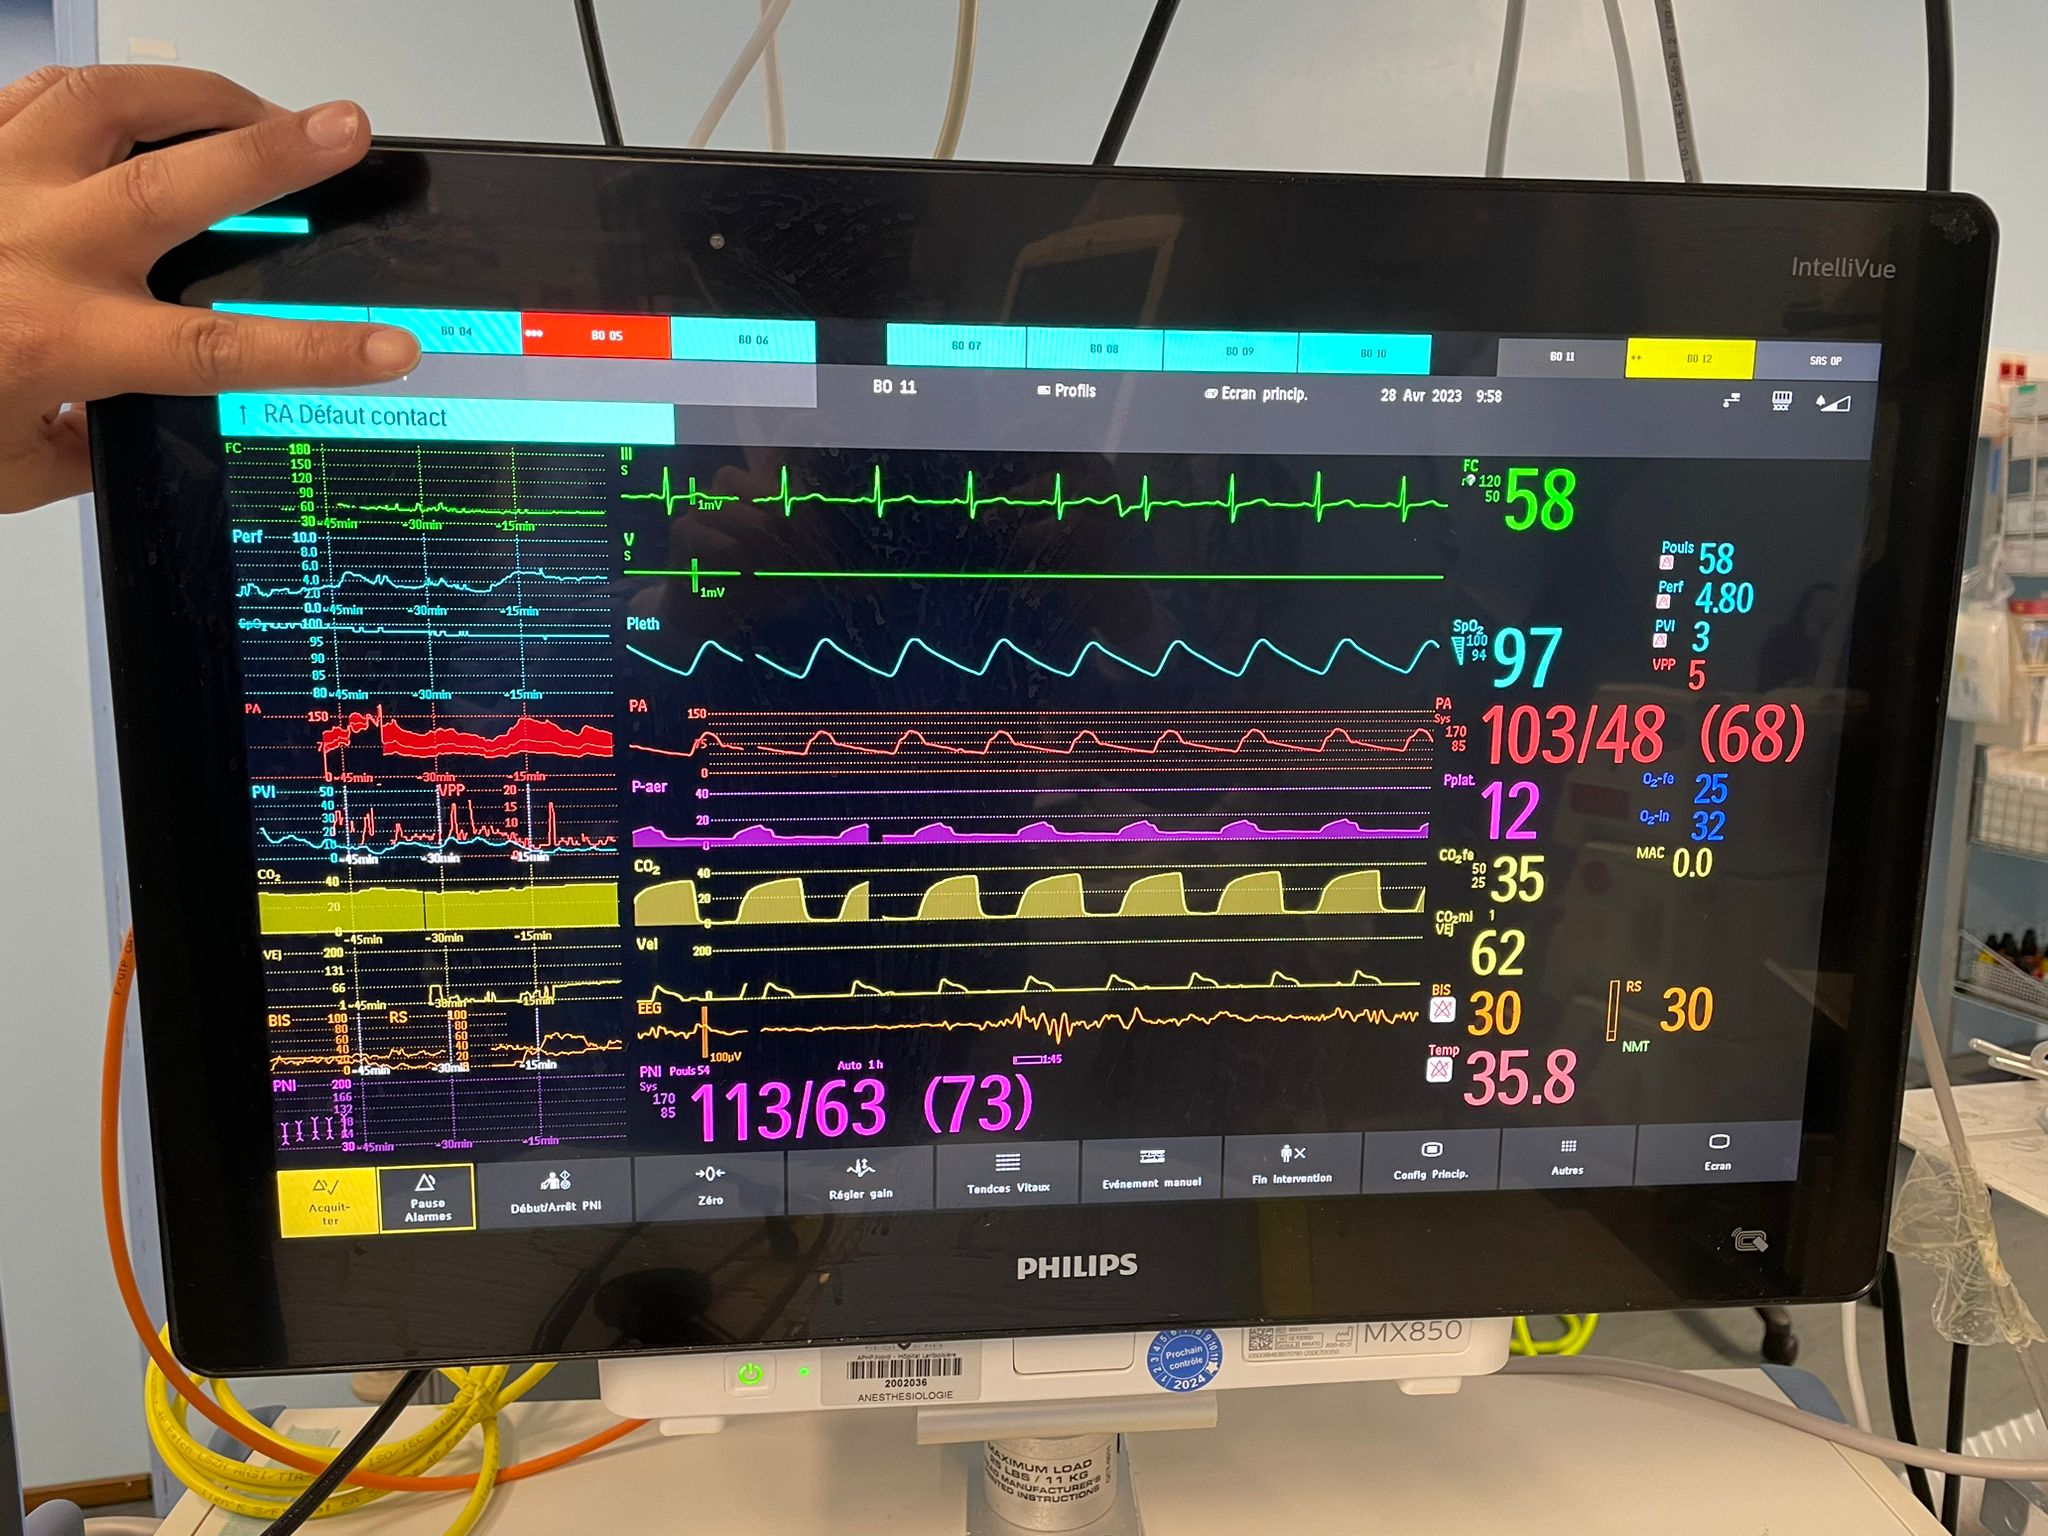
\includegraphics[
            width=1.16\paperwidth
        ]{GA_monitor_1}
    \end{picture}
}
\frame{
    \frametitle{General Anesthesia recordings}


    \begin{tikzpicture}[overlay, remember picture]
            \node[anchor=center, white, xshift=-32ex, yshift=-6em] at (current page.north) (ECG) {\highlight[shadow=false]{\Large \bf ECG}};
            \node[anchor=center, white, xshift=-13ex, yshift=-7.5em] at (current page.north) (ECG_head) {};
            \draw[->, very thick, white] (ECG.east) -- (ECG_head);

            \node[anchor=center, white, xshift=-32ex, yshift=-9.5em] at (current page.north) (Pleth) {\highlight[shadow=false]{\Large \bf Pleth.}};
            \node[anchor=center, white, xshift=-11ex, yshift=-10.5em] at (current page.north) (Pleth_head) {};
            \draw[->, very thick, white] (Pleth.east) -- (Pleth_head);

            \node[anchor=center, white, xshift=-32ex, yshift=-13.5em] at (current page.north) (Resp) {\highlight[shadow=false]{\Large \bf Resp.}};
            \node[anchor=center, white, xshift=-7ex, yshift=-15em] at (current page.north) (Resp_head) {};
            \draw[->, very thick, white] (Resp.east) -- (Resp_head);

            \node[anchor=center, white, xshift=-32ex, yshift=-16.5em] at (current page.north) (EEG) {\highlight[shadow=false]{\Large \bf EEG}};
            \node[anchor=center, white, xshift=-5ex, yshift=-17.5em] at (current page.north) (EEG_head) {};
            \draw[->, very thick, white] (EEG.east) -- (EEG_head);
            \node[anchor=north west, xshift=18ex, yshift=-6em] at (current page.north) {
                \highlight[shadow=false]{Indicators}
            };

    \end{tikzpicture}
}
}

\frame{
    \frametitle{AI-powered General Anesthesia}

    \begin{columns}
        \column{.4\textwidth}
        \centering
        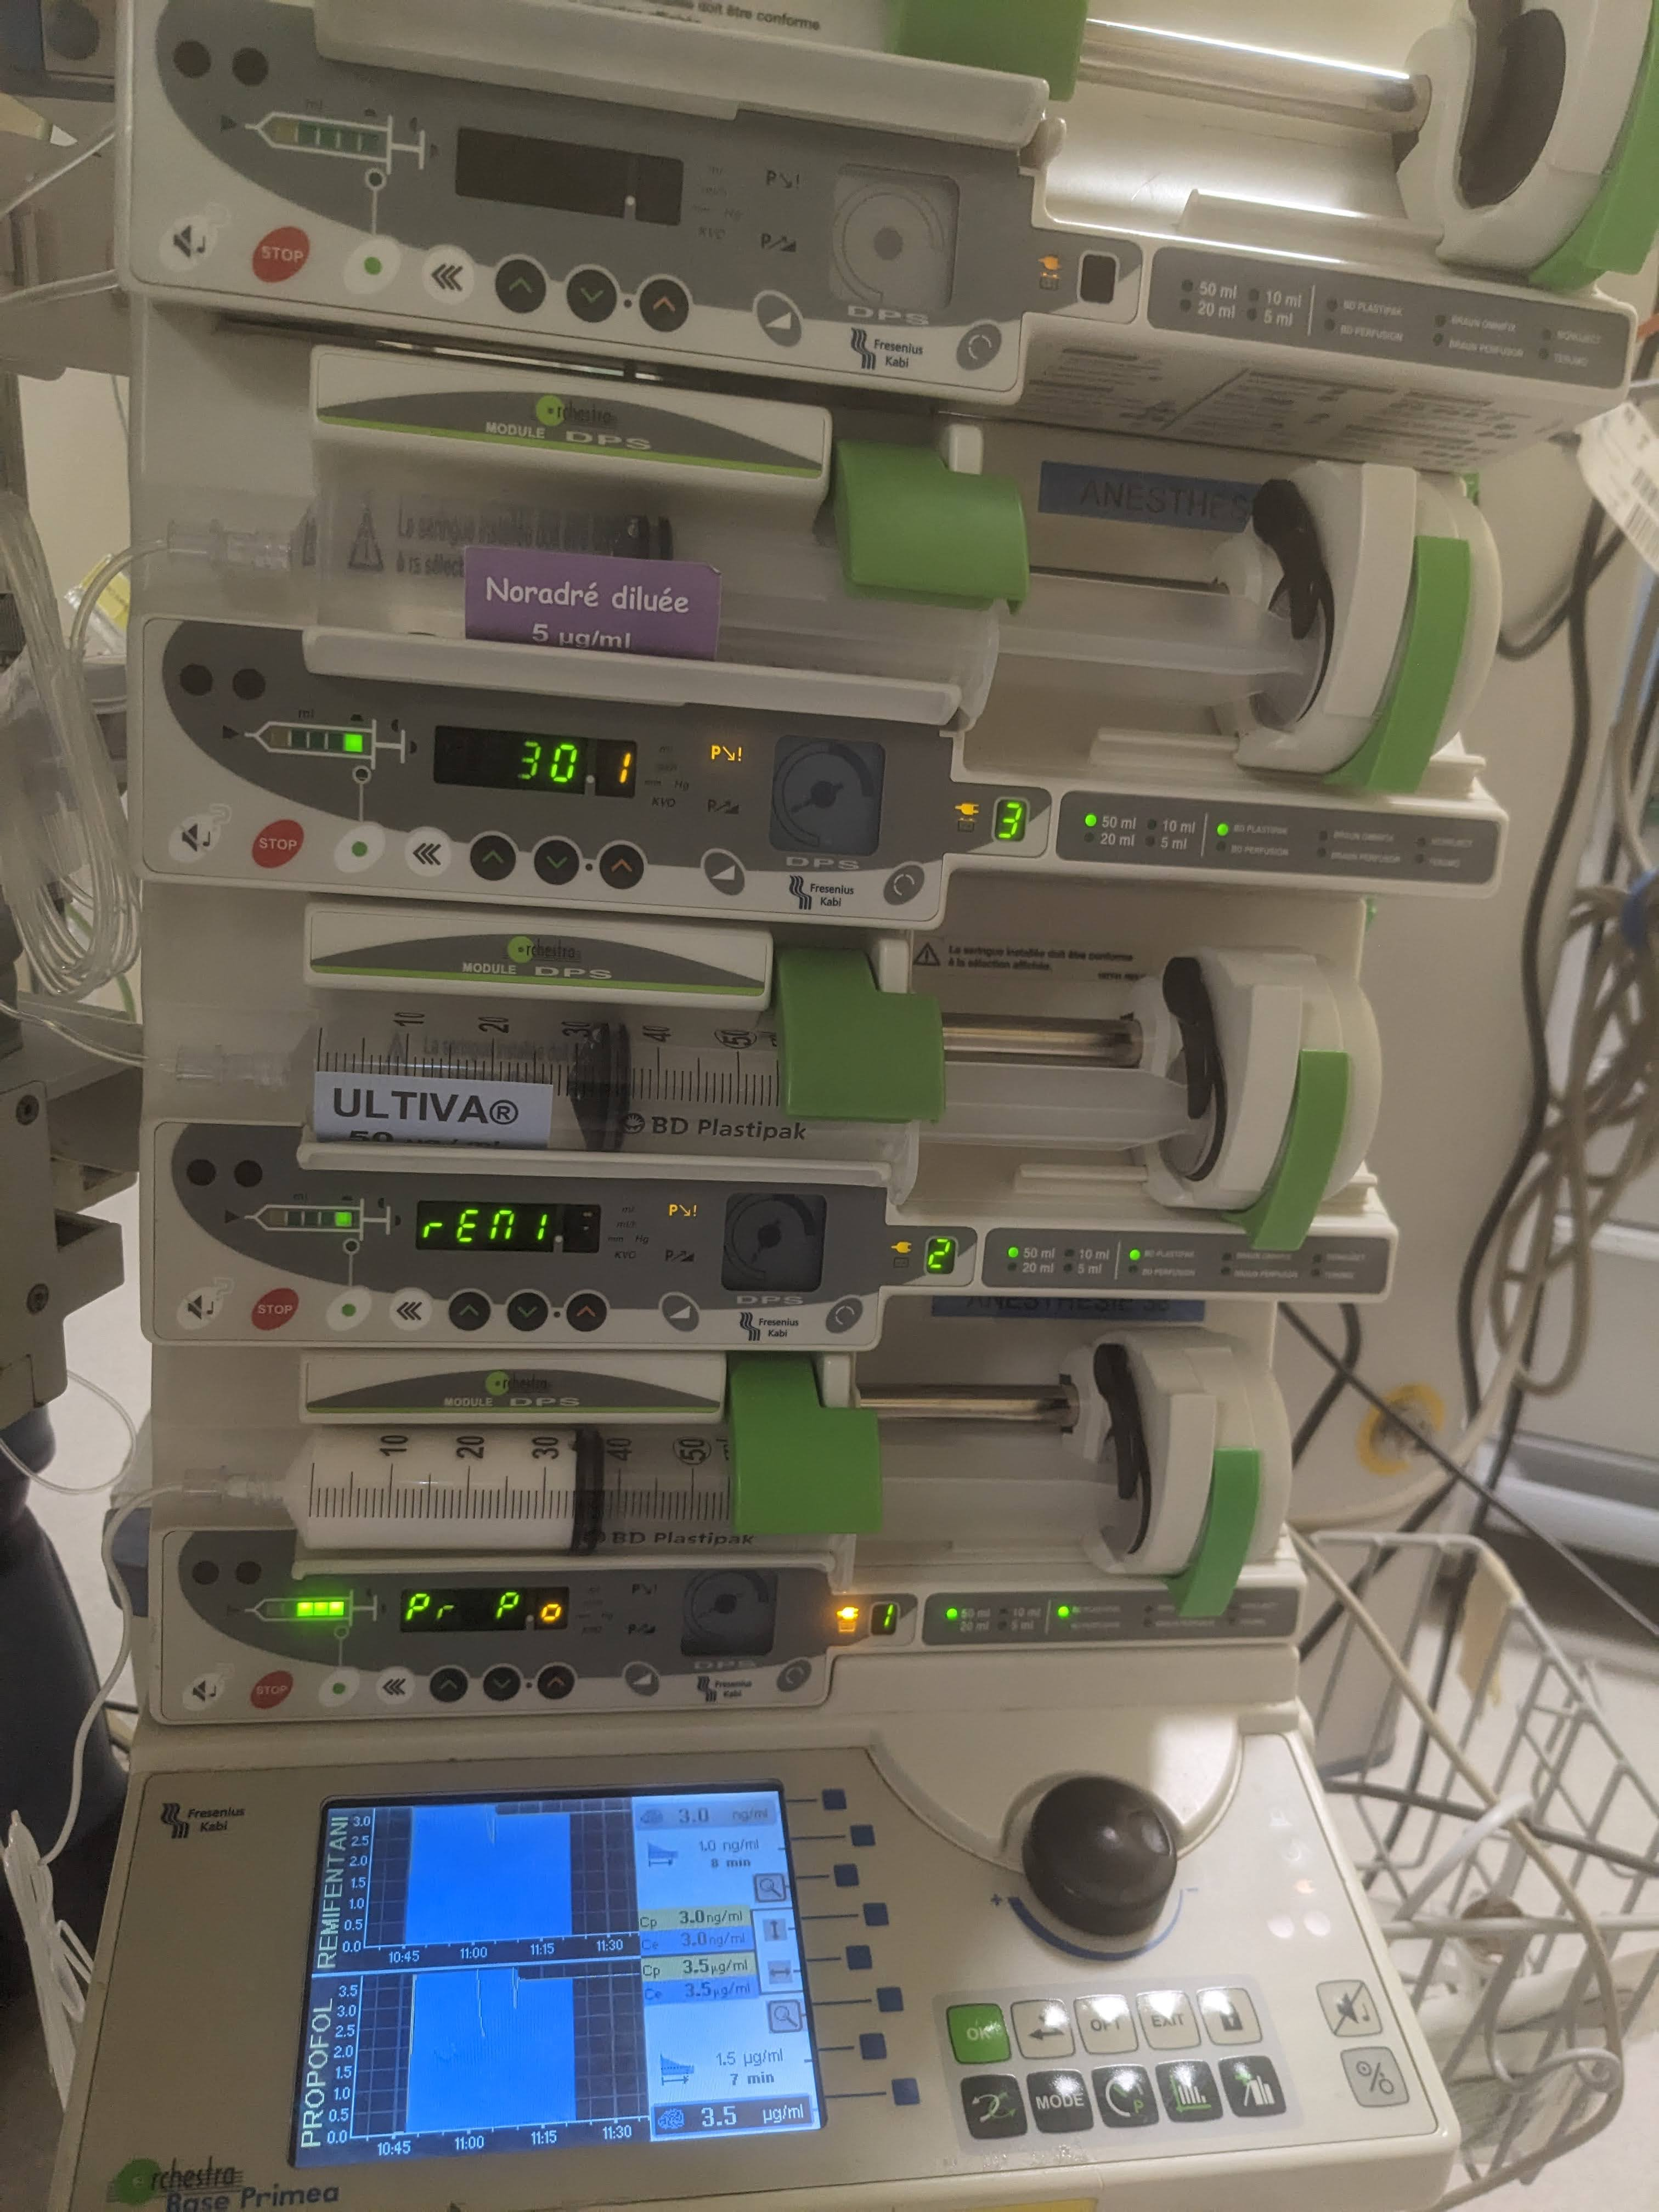
\includegraphics[width=.7\textwidth]{seringe1}\\[1em]
        \highlight{\parbox{.7\textwidth}{
            APHP Database\\
            \normalfont \normalcolor
            46k records; 25Tb\\
            All procedure types
        }}
        \vskip1em
        \includegraphics[height=2em]{logo_APHP}
        \column{.6\textwidth}
        Anesthetists make {\bf decisions} based on these
        indicators.\\[1em]

        \begin{itemize}\itemsep.5em
            \color{black}\normalfont
            \item Instantaneous snapshot,
            \item Reading needs expertise,
            \item Not personalized.
        \end{itemize}
        \vskip1em
        The MASCOT team (F. Vallée) from APHP (Paris hospital) have been collecting GA recordings for 5 years.
        \vskip2em
        \strongpoint{Can we leverage AI to better drive GA?}
    \end{columns}


}

%------------------------------------------------------------------------------
\frame[t]{
    \frametitle[t]{Recent successes in AI: Foundation Models}

    \begin{columns}[T]
        \column{.2\textwidth}\centering
        
\includegraphics[height=4em]{logo_chatGPT}\\
        \textbf{ChatGPT}
        \column{.2\textwidth}\centering
        
\includegraphics[height=4em]{logo_copilot}\\
        \textbf{Copilot}
        \column{.2\textwidth}\centering
        
\includegraphics[height=4em]{logo_midjourney}\\
        \textbf{Midjourney}
    \end{columns}
    \vskip1em
    {\centering \large What do they have in common?\\}

    \pause

    \vskip1em
    \begin{columns}[T]
        \techterm{Self-supervised Pretraining}
        \techterm{Transformers}
        \techterm{Fine-tuning}
    \end{columns}
    \vskip1em
    \myitem{} Capture $\mathbb P(X)$ through interaction between {\bf tokens}.

    \only<3>{
        \vskip1em
        {\bf Challenges for signals:}\\[1em]
        \begin{itemize}\itemsep.5em
            \item What are the tokens for the physiological signals?
            \item Databases are smaller than Text and Images,
        \end{itemize}
    }


}

%------------------------------------------------------------------------------
{
\usebackgroundtemplate{
    \begin{picture}(400, 300)(45, 0)
        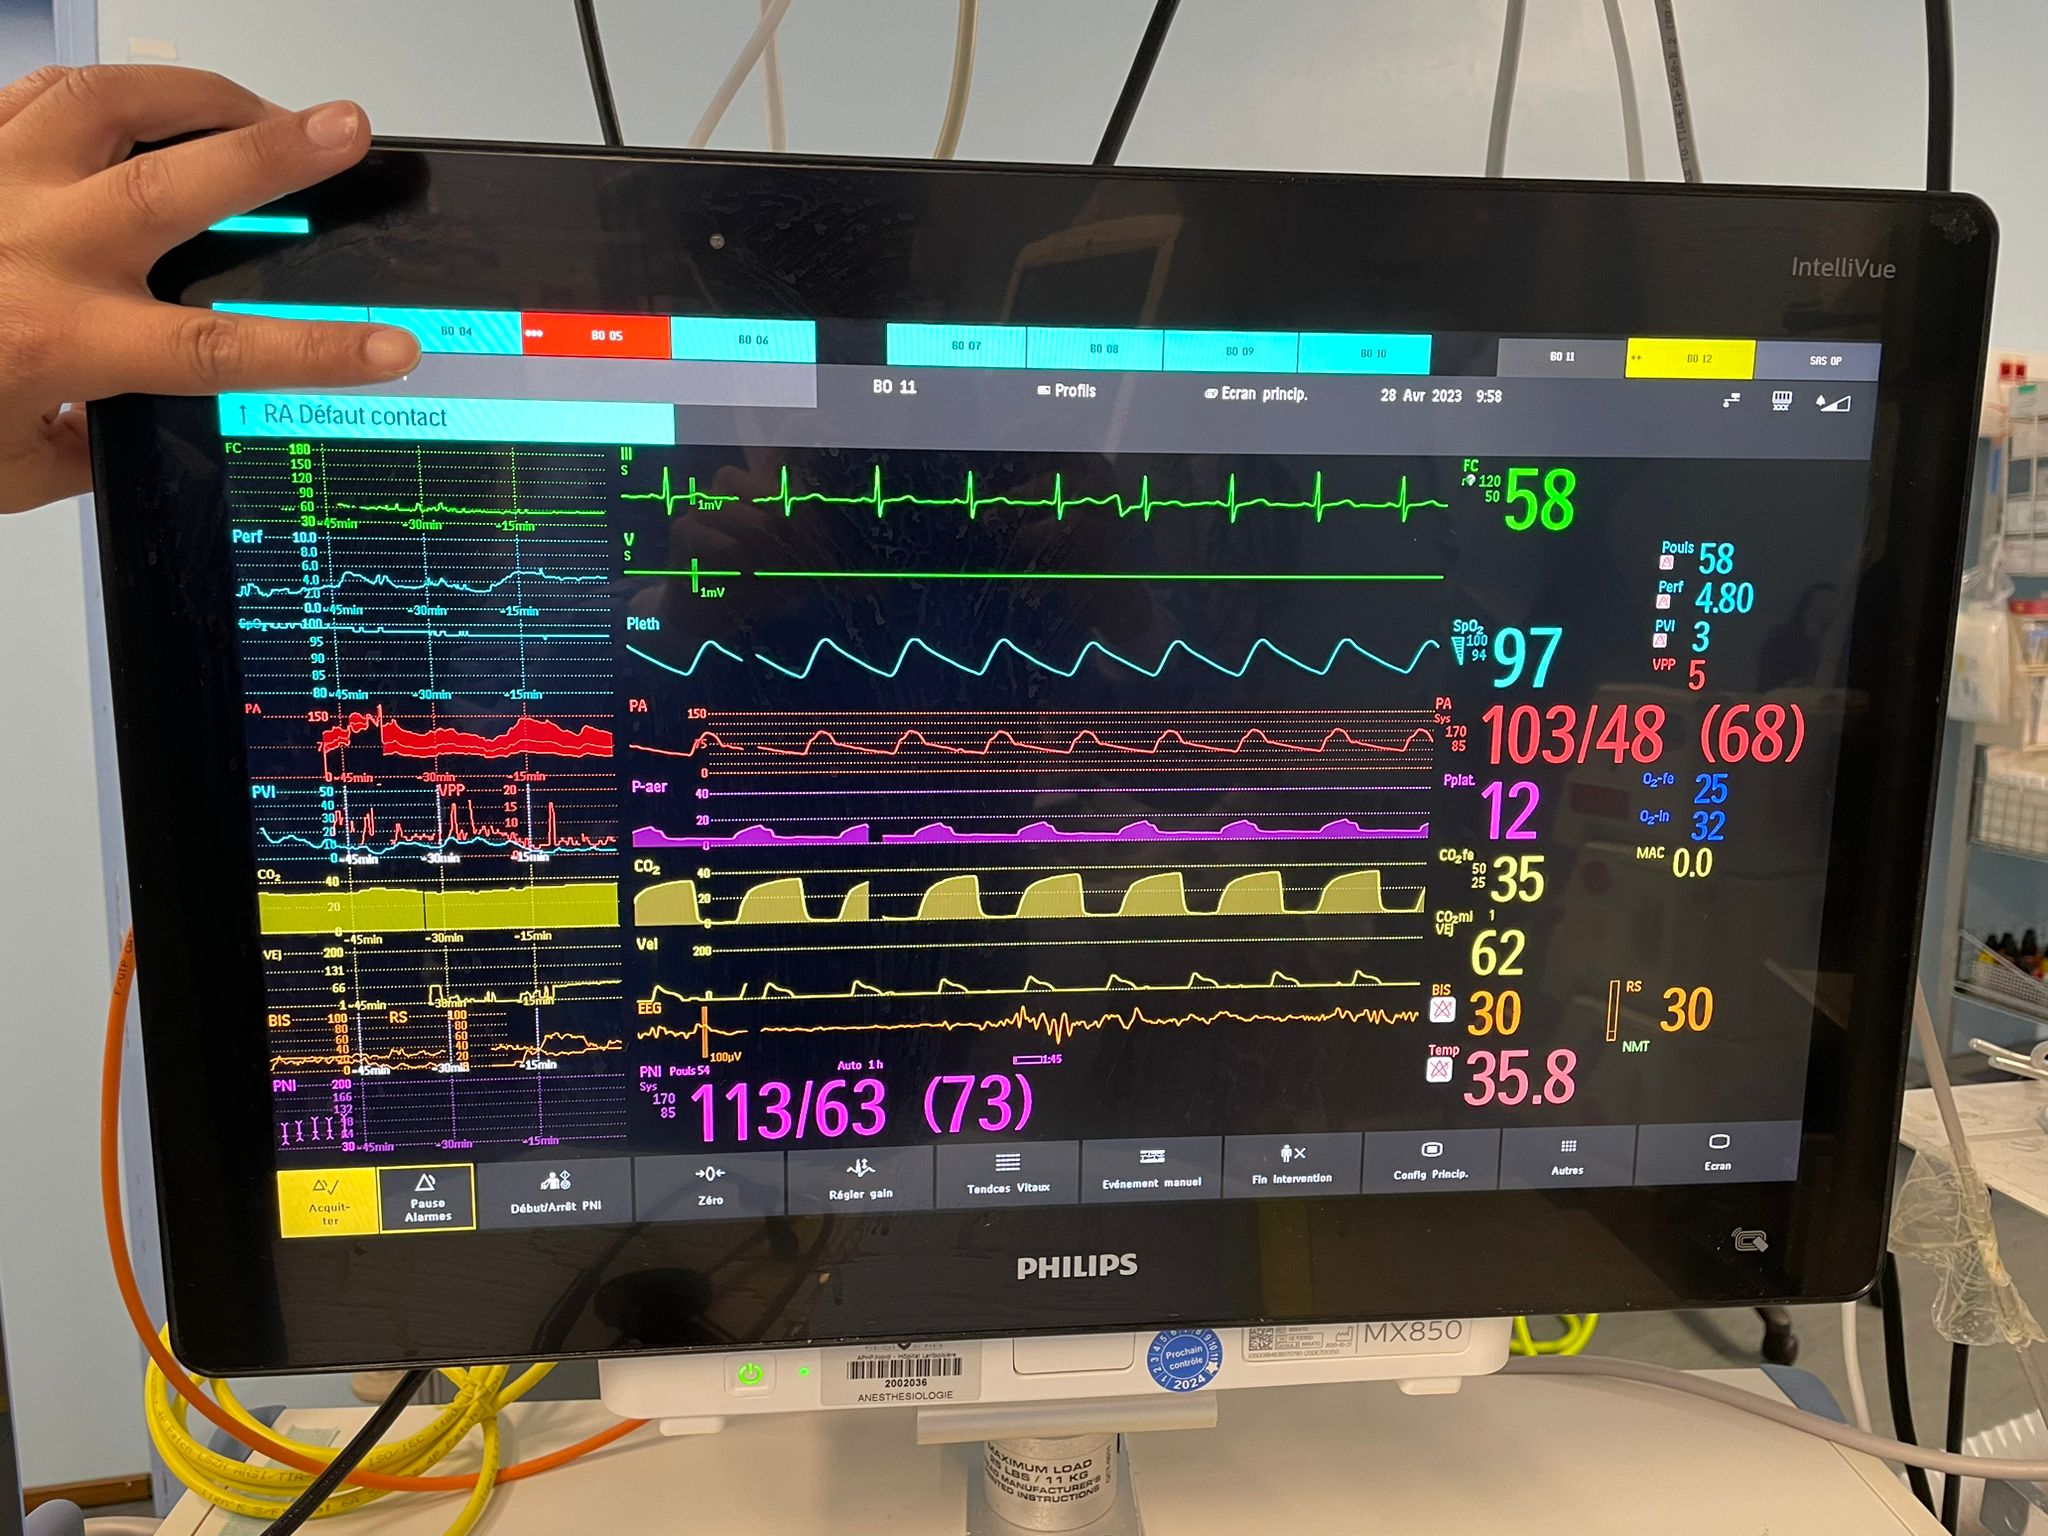
\includegraphics[
            width=1.16\paperwidth
        ]{GA_monitor_1}
    \end{picture}
}
\frame{
    \frametitle{Signals' tokens: Patterns and Events}


    \setbeamercolor{events}{bg=darkred!50}
    \begin{tikzpicture}[overlay, remember picture]

        \node[anchor=west, yshift=7em] at (current page.west)
            (patterns) {\highlight[shadow=false]{Signal's patterns}};

        \node[anchor=west, yshift=-2.5em] at (patterns.west) (ECG) {\highlight[shadow=false]{\color{black}\normalfont Heartbeat}};
        \node[anchor=center, lightblue!70, xshift=-13ex, yshift=-7.5em] at (current page.north) (ECG_head) {};
        \draw[->, very thick, lightblue!70] (ECG.east) -- (ECG_head);

        \node[rectangle, lightblue!70, draw=lightblue!70, very thick,
            minimum width=5ex,
            minimum height=2em, xshift=-9ex, yshift=-7.8em]
                at (current page.north) {};

        \node[anchor=west, yshift=-5em] at (patterns.west) (Pleth) {\highlight[shadow=false]{\color{black}\normalfont  Dicrote}};
        \node[anchor=center, lightblue!70, xshift=-9ex, yshift=-10.5em] at (current page.north) (Pleth_head) {};
        \draw[->, very thick, lightblue!70] (Pleth.east) -- (Pleth_head);

        \node[rectangle, lightblue!70, draw=lightblue!70, very thick,
            minimum width=4ex,
            minimum height=2em, xshift=-7ex, yshift=-10.8em]
                at (current page.north) {};

        \node[anchor=west, yshift=-7.5em] at (patterns.west) (Resp) {\highlight[shadow=false]{\color{black}\normalfont  Cycle}};
        \node[anchor=center, lightblue!70, xshift=-8ex, yshift=-15em] at (current page.north) (Resp_head) {};
        \draw[->, very thick, lightblue!70] (Resp.east) -- (Resp_head);

        \node[rectangle, lightblue!70, draw=lightblue!70, very thick,
            minimum width=4ex,
            minimum height=2em, xshift=-6ex, yshift=-15.5em]
                at (current page.north) {};

        \node[anchor=west, yshift=-10em] at (patterns.west) (EEG) {\highlight[shadow=false]{\color{black}\normalfont  Brain waves}};
        \node[anchor=center, lightblue!70, xshift=-5ex, yshift=-17.5em] at (current page.north) (EEG_head) {};
        \draw[->, very thick, lightblue!70] (EEG.east) -- (EEG_head);

        \node[rectangle, lightblue!70, draw=lightblue!70, very thick,
            minimum width=6ex,
            minimum height=1.3em, xshift=-2ex, yshift=-17.8em]
                at (current page.north) {};




        \node[anchor=east, xshift=-3em, yshift=7em] at (current page.east)
            (events) {\highlight[shadow=false, col=events,c=white]{
                External events
            }};
        \node[anchor=east, yshift=-3.5em] at (events.east)
            {\highlight[shadow=false,col=events,c=black]{
                \normalfont Drug injection
            }};
        \node[anchor=east, yshift=-7em] at (events.east)
            {\highlight[shadow=false,col=events,c=black]{
                \normalfont Surgery acts
            }};
        \node[anchor=east, yshift=-10.5em] at (events.east)
            {\highlight[shadow=false,col=events,c=black]{
                \normalfont Adverse outcomes
            }};

        \only<2>{
            \node[anchor=west, yshift=-8em] at (current page.west)
            {\highlight[shadow=false,col=events,c=white]{
                Physiological events
            }};
        }

    \end{tikzpicture}
}
}


%------------------------------------------------------------------------------

\begin{frame}[t]{Signals' tokens: Events}

    \vskip-1em
    \begin{columns}[T]
        \column{.5\textwidth}
        \centering
        \begin{tikzpicture}
                \node[inner sep=0em, outer sep=0em] (img) {\includegraphics[width=.9\linewidth]{meg_signal}};
                \path let
                  \p1=($(img.north) - (0, 1em)$), \p2=(img.south)
                  in
                  node {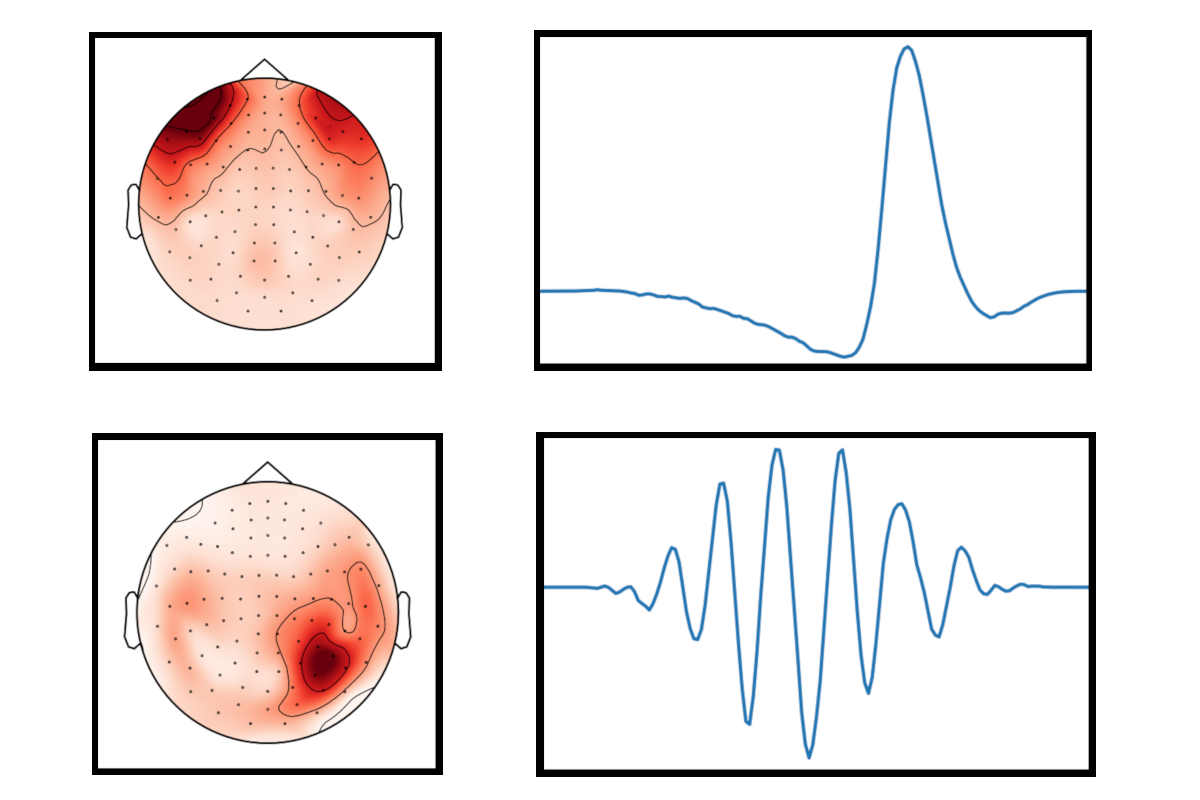
\includegraphics[height=\y1-\y2]{meg_dict}};
            \end{tikzpicture}\\
        {\large MEG}\\[1em]
        \begin{tikzpicture}
            \node[inner sep=0em, outer sep=0em] (img) {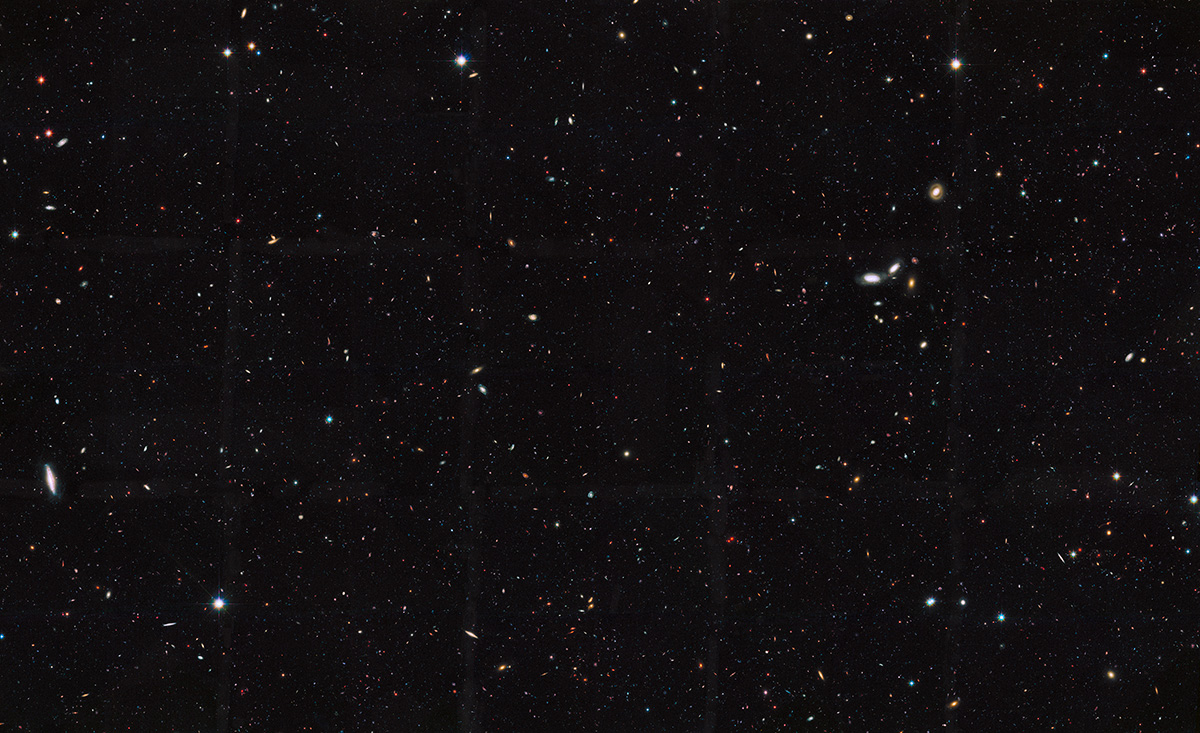
\includegraphics[width=.9\linewidth]{Hubble}};
            \path let
                \p1=($(img.north) - (0, 1em)$), \p2=(img.south)
                in
                node {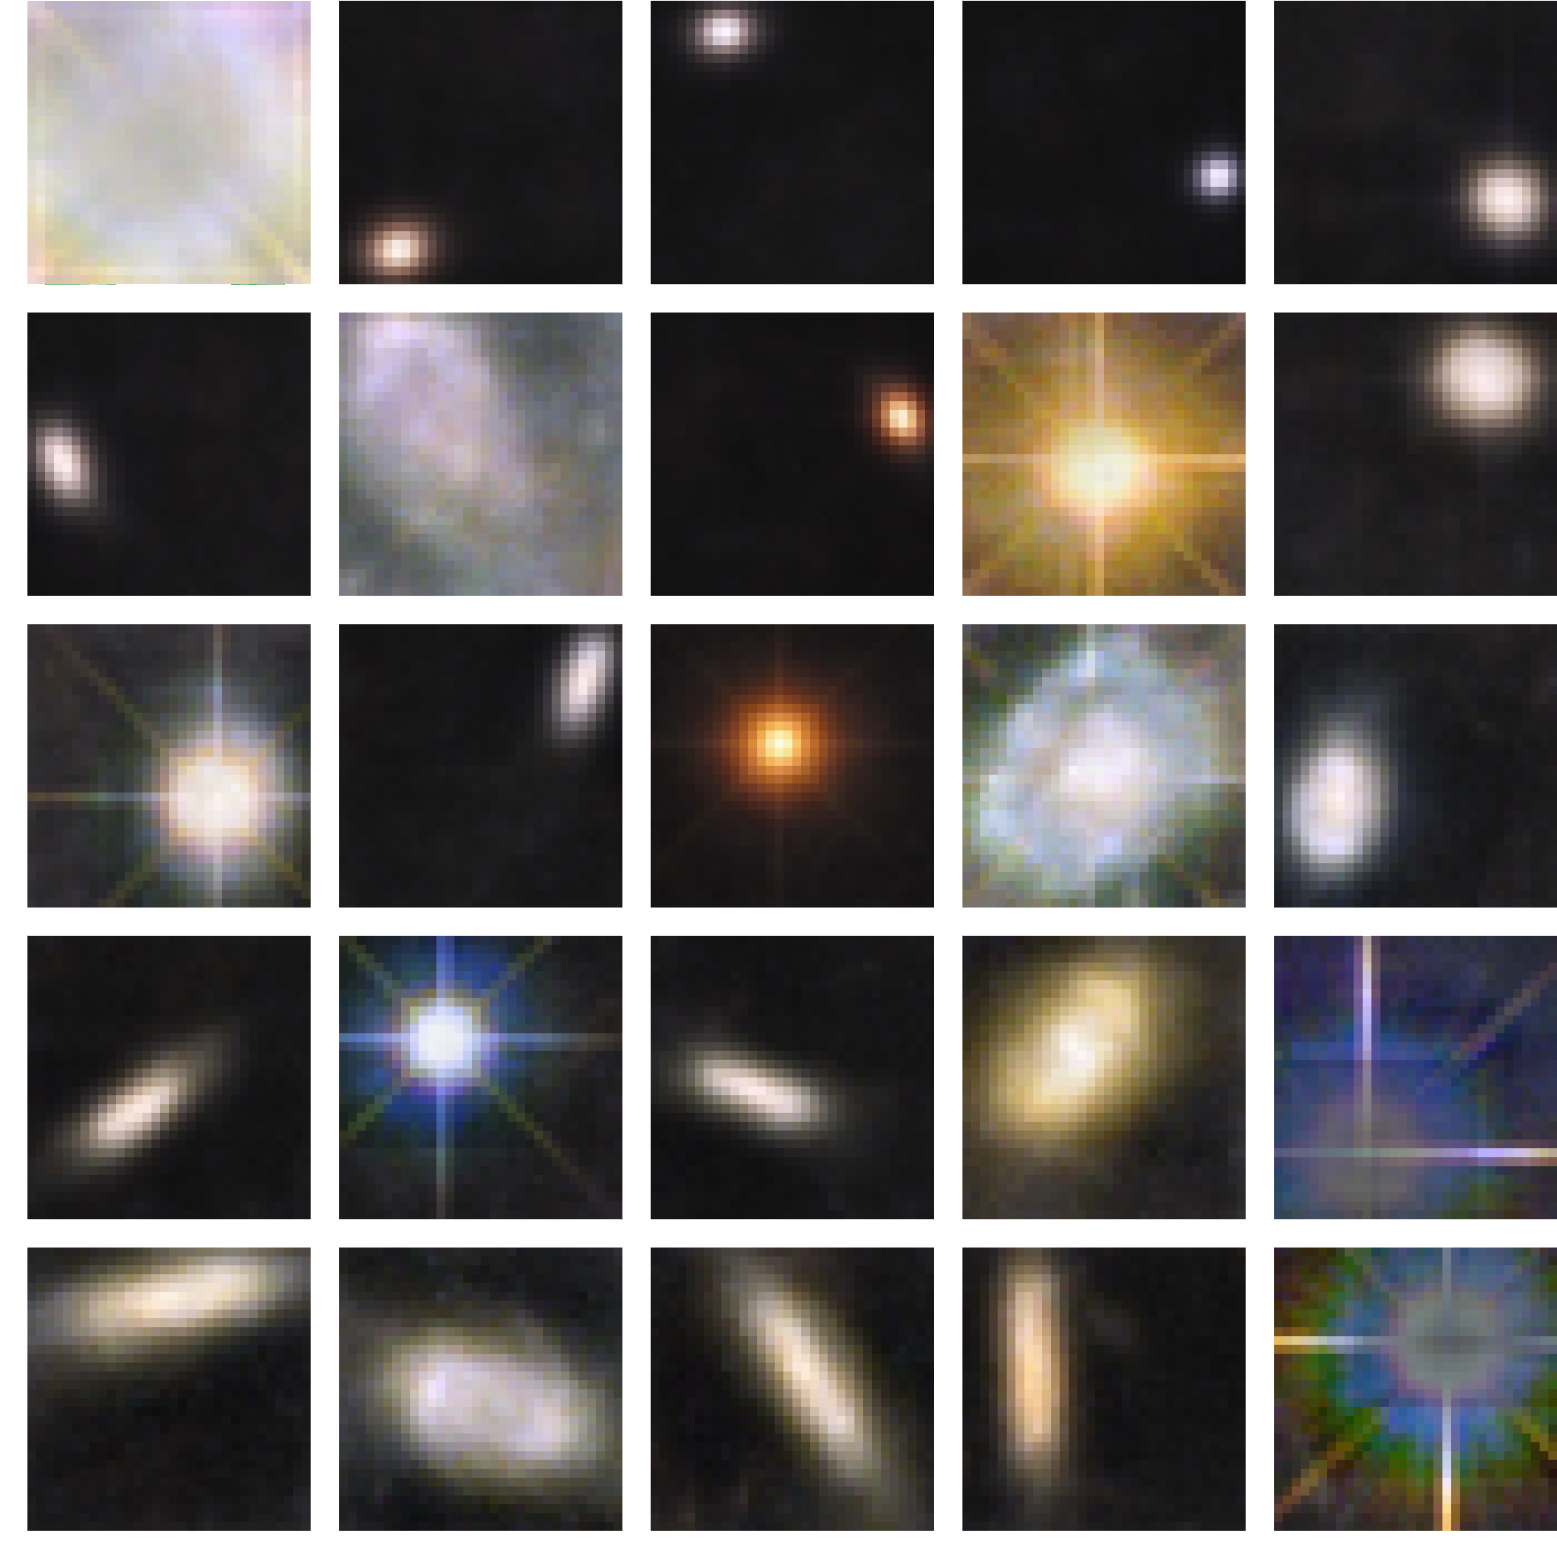
\includegraphics[height=\y1-\y2]{Hubble_dict}};
        \end{tikzpicture}\\
        {\large Astronomy}\\
    \column{.5\textwidth}
        \centering
        \begin{tikzpicture}
            \node[inner sep=0em, outer sep=0em] (img) {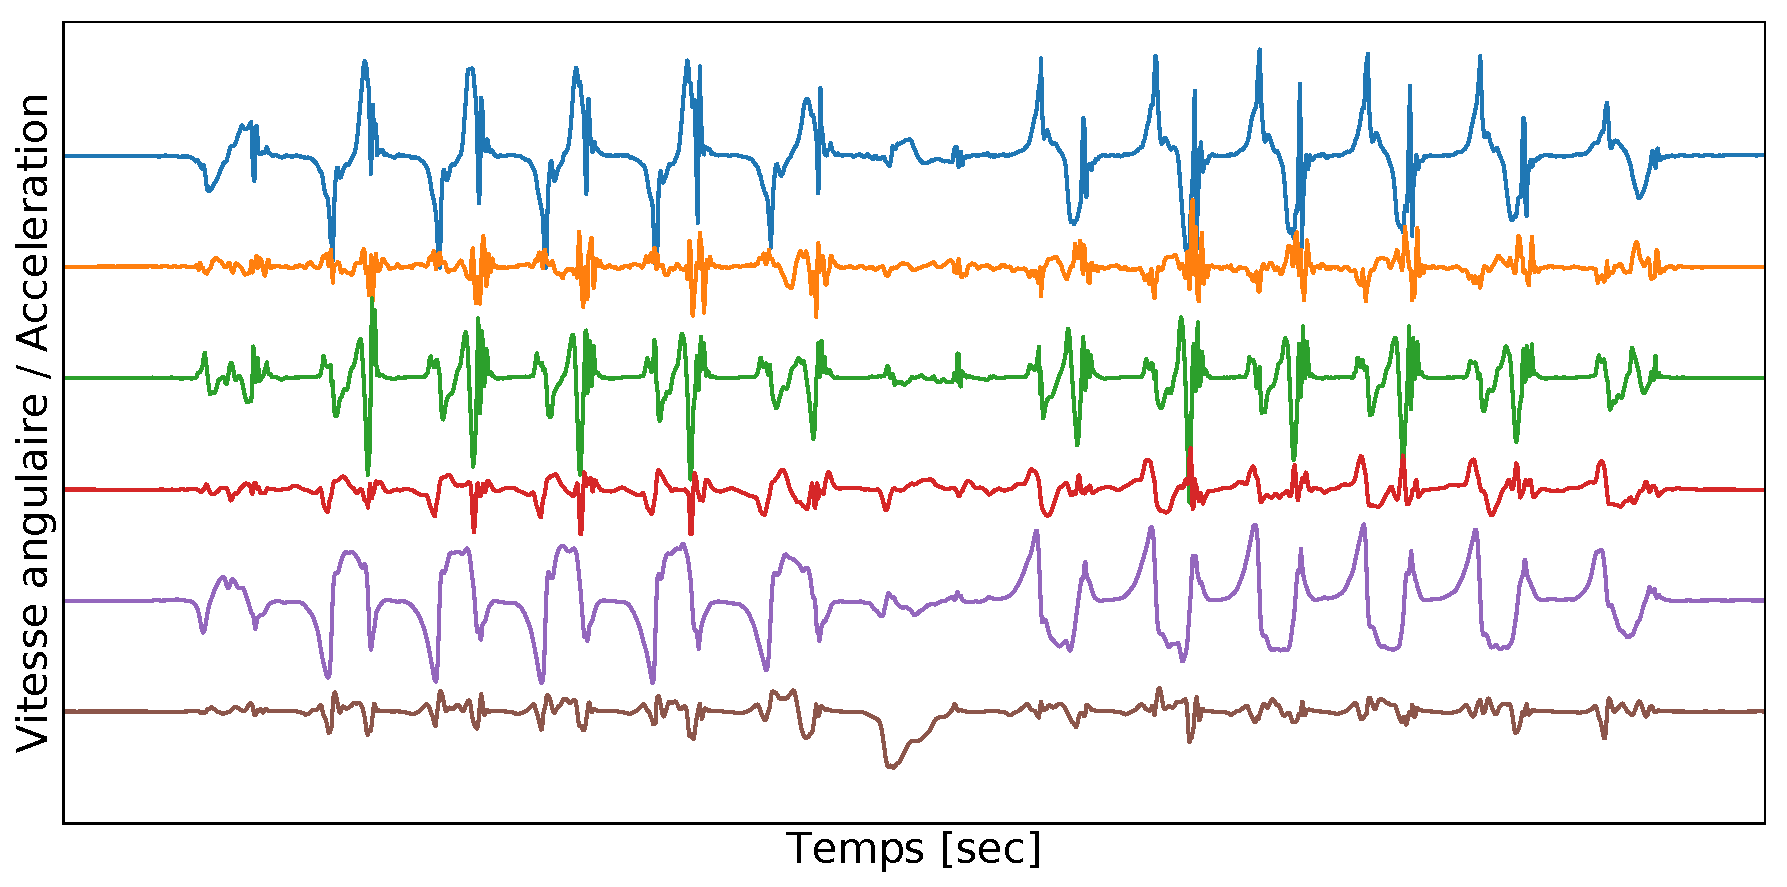
\includegraphics[width=.9\linewidth]{accelero}};
            \path let
                \p1=($(img.north) - (0, 1em)$), \p2=(img.south)
                in
                node {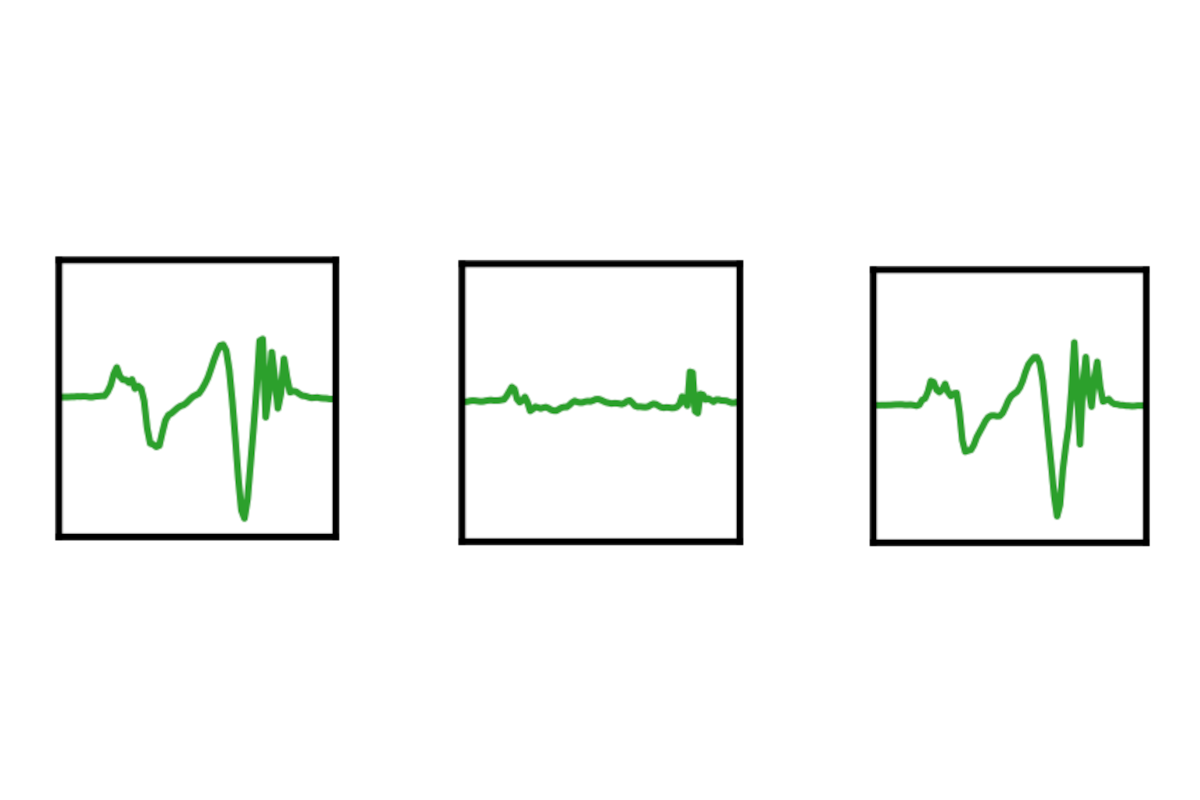
\includegraphics[height=\y1-\y2]{accelero_dict}};
        \end{tikzpicture}\\
        {\large Gait analysis}\\[1em]
        \begin{tikzpicture}
            \node[inner sep=0em, outer sep=0em] (img) {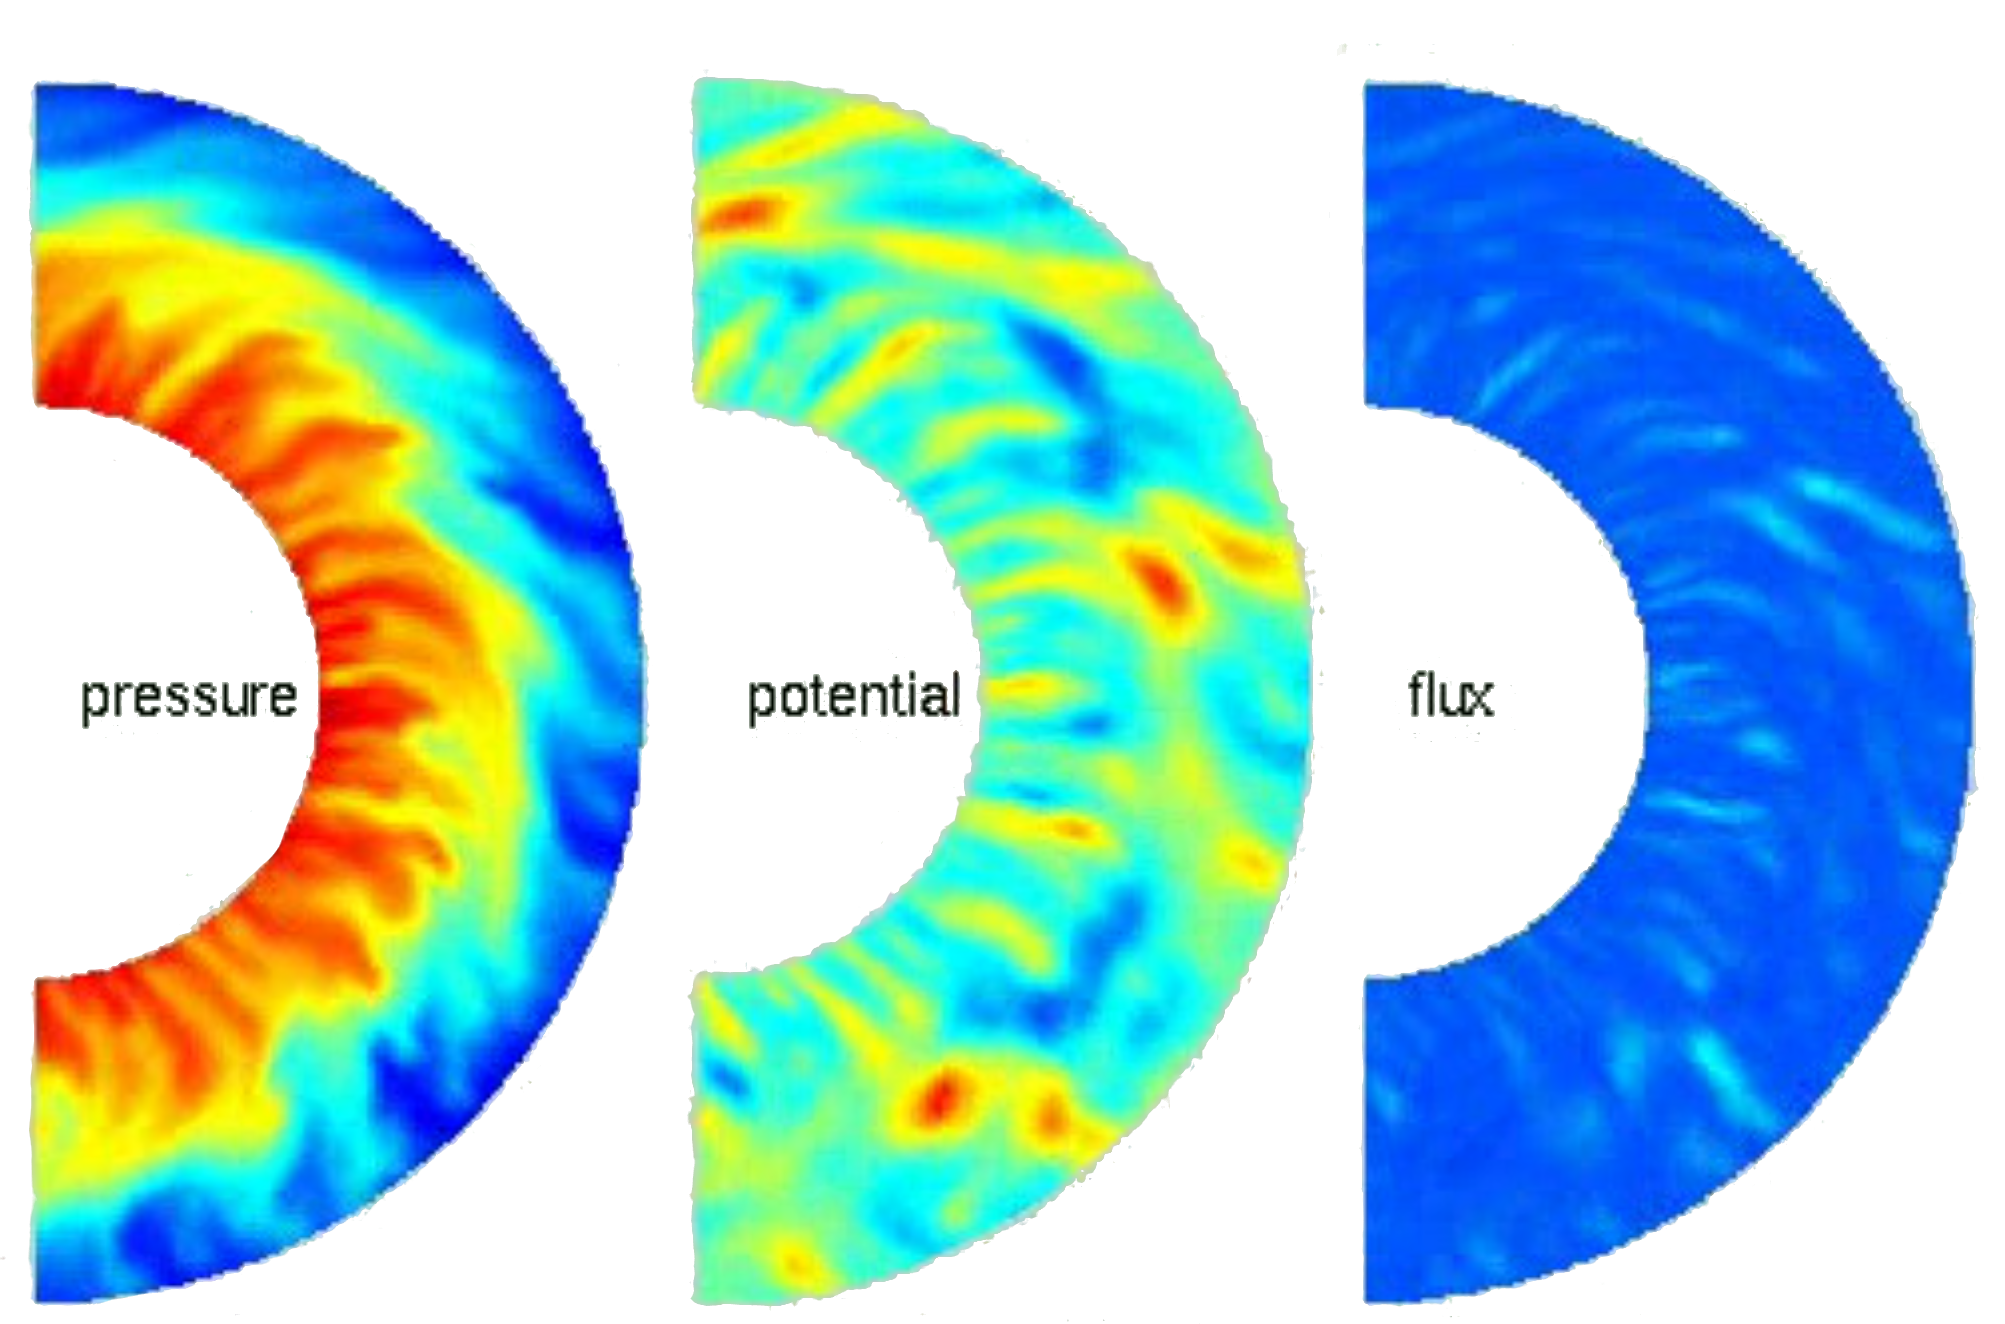
\includegraphics[width=.9\linewidth]{tokamak}};
            \path let
                \p1=($(img.north) - (0, 1em)$), \p2=(img.south)
                in
                node {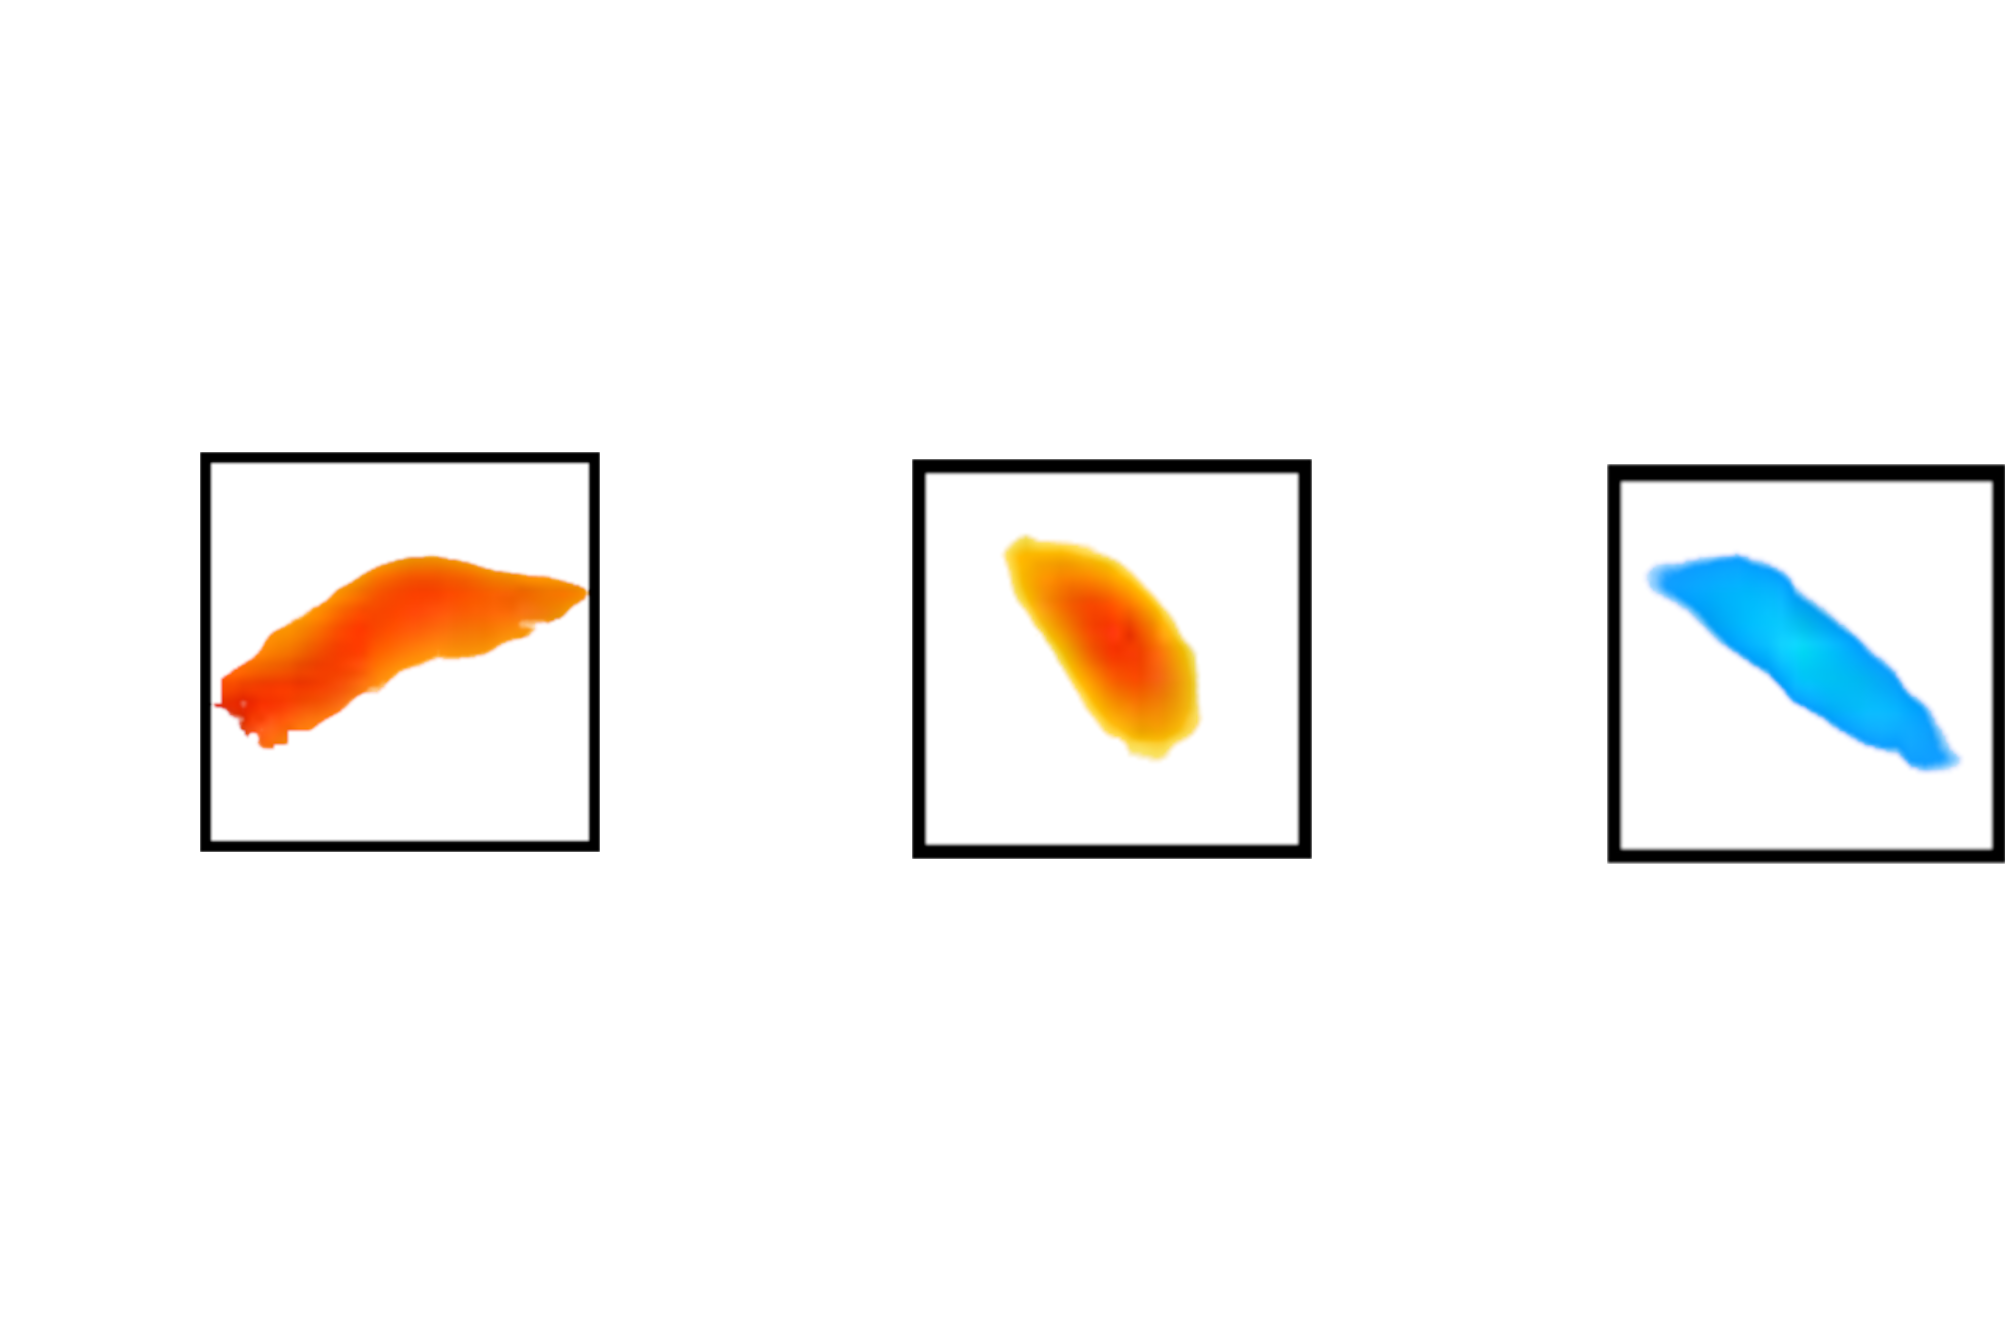
\includegraphics[height=\y1-\y2]{tokamak_dict}};
        \end{tikzpicture}\\
        {\large Plasma Simulation}\\

    \end{columns}

    \visible<2>{\vskip-14em
    \centering
    \highlight{\parbox{.4\textwidth}{
        \centering
        Physical Events\\
        are often characterized by
        Recurring Patterns
    }}\\
    }
\end{frame}


%------------------------------------------------------------------------------

\frame{
    \frametitle{EULPS: Event-based unsupervised learning for Physiological Signals}

    {\bf Hyp.:} Events' time distribution $\mathbb P(\{t_k\}_k)$ is much simpler than $\mathbb P(X)$.\\[1em]

    % {\bf Two roads:}
    % \begin{columns}[T]
    %     \column{.5\textwidth}
    %     {\centering\highlight{Deep Learning}\\}
    %     \vskip.5em
    %     \begin{itemize}
    %         \item Very expressive,
    %         \item Require very large database,
    %         \item Black-box.
    %     \end{itemize}
    %     \column{.5\textwidth}
    %     {\centering\highlight{Parametric Model}\\}
    %     \vskip.5em
    %     \begin{itemize}
    %         \item Limited fine-tuning,
    %         \item Sample efficient,
    %         \item Explicit.
    %     \end{itemize}
    % \end{columns}

    % \strongpoint{From parametric to deep models}

    % TODO: here I need to explain the issue!!

    \begin{block}{\bf EULPS Goal}
        Model the Distribution of Events for Physiological Signals.
    \end{block}

    \vskip1em
    {\bf Challenge:} Need to find events and model their distribution jointly.\\[1em]

    {\centering
\includegraphics[width=.8\textwidth]{finding_events}\\[1em]}

    {\bf Approach:} from parametric to deep models.
}

%------------------------------------------------------------------------------

\frame{
    \frametitle{WP1: Parametric PP to model Physiological Signals Events}

    \begin{block}{\bf Challenge 1}
        Which parametric models for Physiological Signals Events?
    \end{block}

    {\bf Idea:} use Point Processes to model the events' distribution $\mathbb P(\{t_k\}_k)$\\[1em]

    \begin{columns}
        \column{.6\textwidth}
        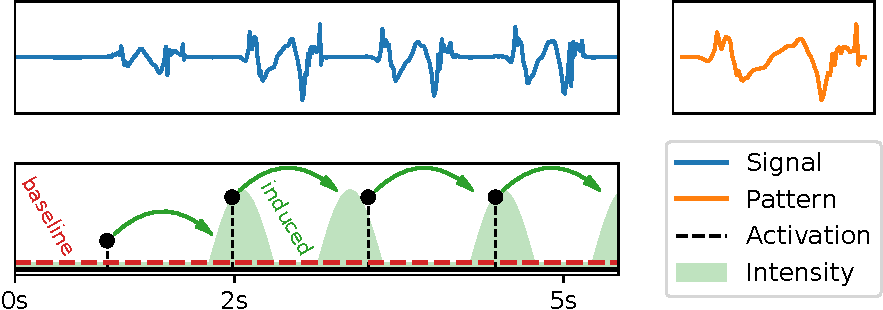
\includegraphics[width=\textwidth]{csc_and_pp}\\
        \column{.4\textwidth}
        \includegraphics[width=\textwidth]{connectivity_default_mode}
    \end{columns}

    \vskip1em
    {\bf Development:} Models beyond Markovian kernels to model uncertainty in space and time and complex events' dependencies.
    % \myitem{} General Parametric Family for temporal, marked and spatial PP.

    \vskip1em
    {\bf Preliminary Studies:} \fakecite{ICLR 2022; ICML 2023}

}

%------------------------------------------------------------------------------

\frame{
    \frametitle{WP2: Event-based unsupervised waveform learning\\for physiological signals}

    \begin{block}{\bf Challenge 2}
        Can we jointly discover the Events and model them?
    \end{block}

    \begin{columns}[T]
        \column{.5\textwidth}
        {\centering
        \highlight{Parametric models}\\[.5em]}
        \hskip-3ex\begin{tikzpicture}
            \node (AM) {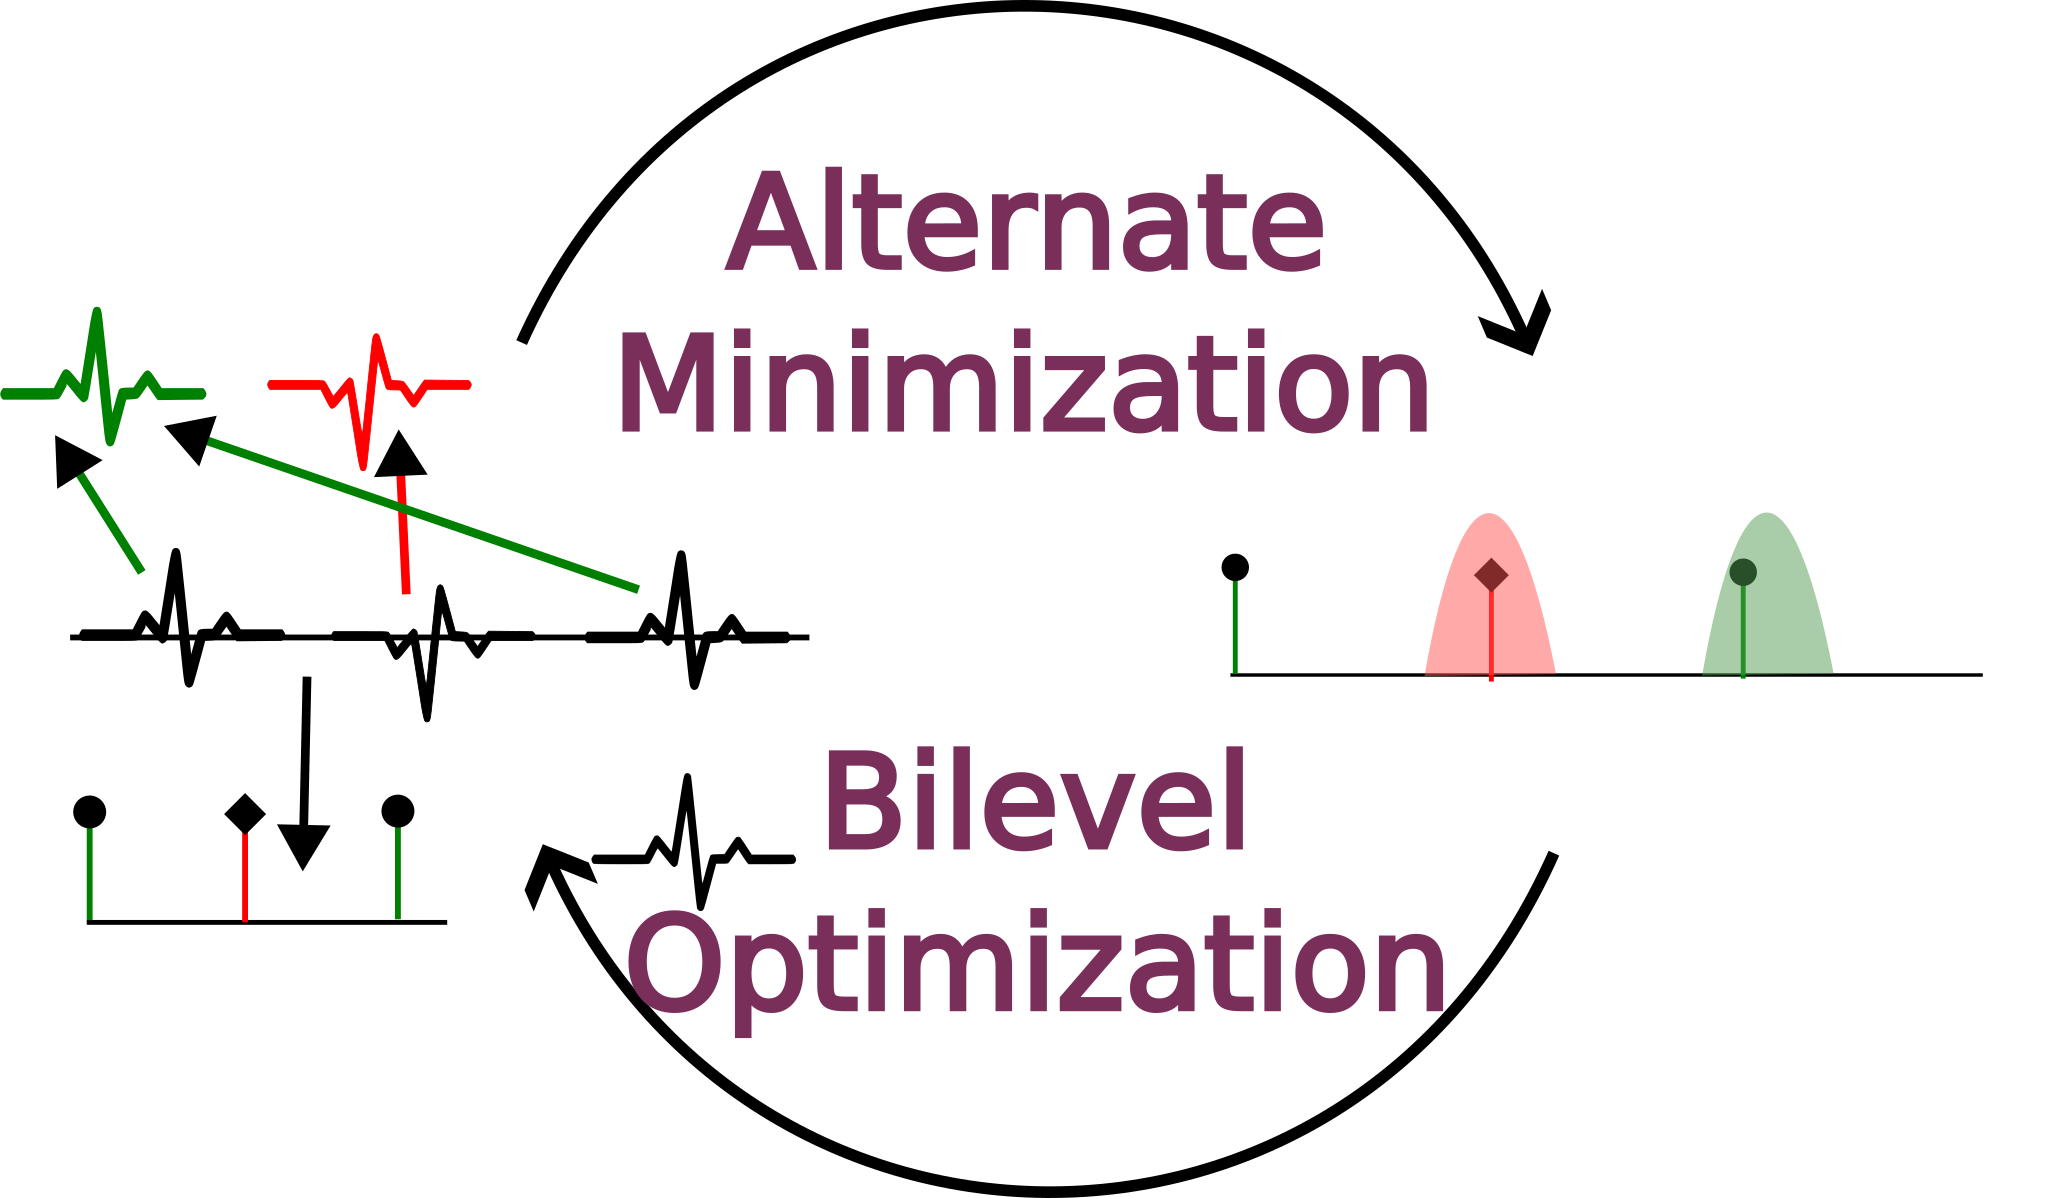
\includegraphics[width=.9\textwidth]{parametric_model}};

            \node[anchor=north west, xshift=-4ex, yshift=1ex] at (AM.north west) {
                \highlight[shadow=false]{\parbox{.28\textwidth}{
                    \tiny \centering Conv. Dictionary Learning
                }}
            };
            \node[anchor=south west, xshift=-4ex, yshift=-1ex] at (AM.south west) {
                \highlight[shadow=false]{\parbox{.28\textwidth}{
                    \tiny \centering Change Points Detection
                }}
            };
            \node[anchor=north east, xshift=1ex, yshift=.5ex] at (AM.north east) {
                \highlight[shadow=false]{\parbox{.23\textwidth}{
                    \tiny \centering Point Process (WP1)
                }}
            };
        \end{tikzpicture}
        % \begin{itemize}
        %     \item Based on Convolutional Dictionary Learning and PP,
        %     \item Use bilevel optimization.
        % \end{itemize}
        \column{.5\textwidth}
        {\centering
        \highlight{Deep Learning models}\\[.5em]}

        \begin{tikzpicture}
            \node (unroll) {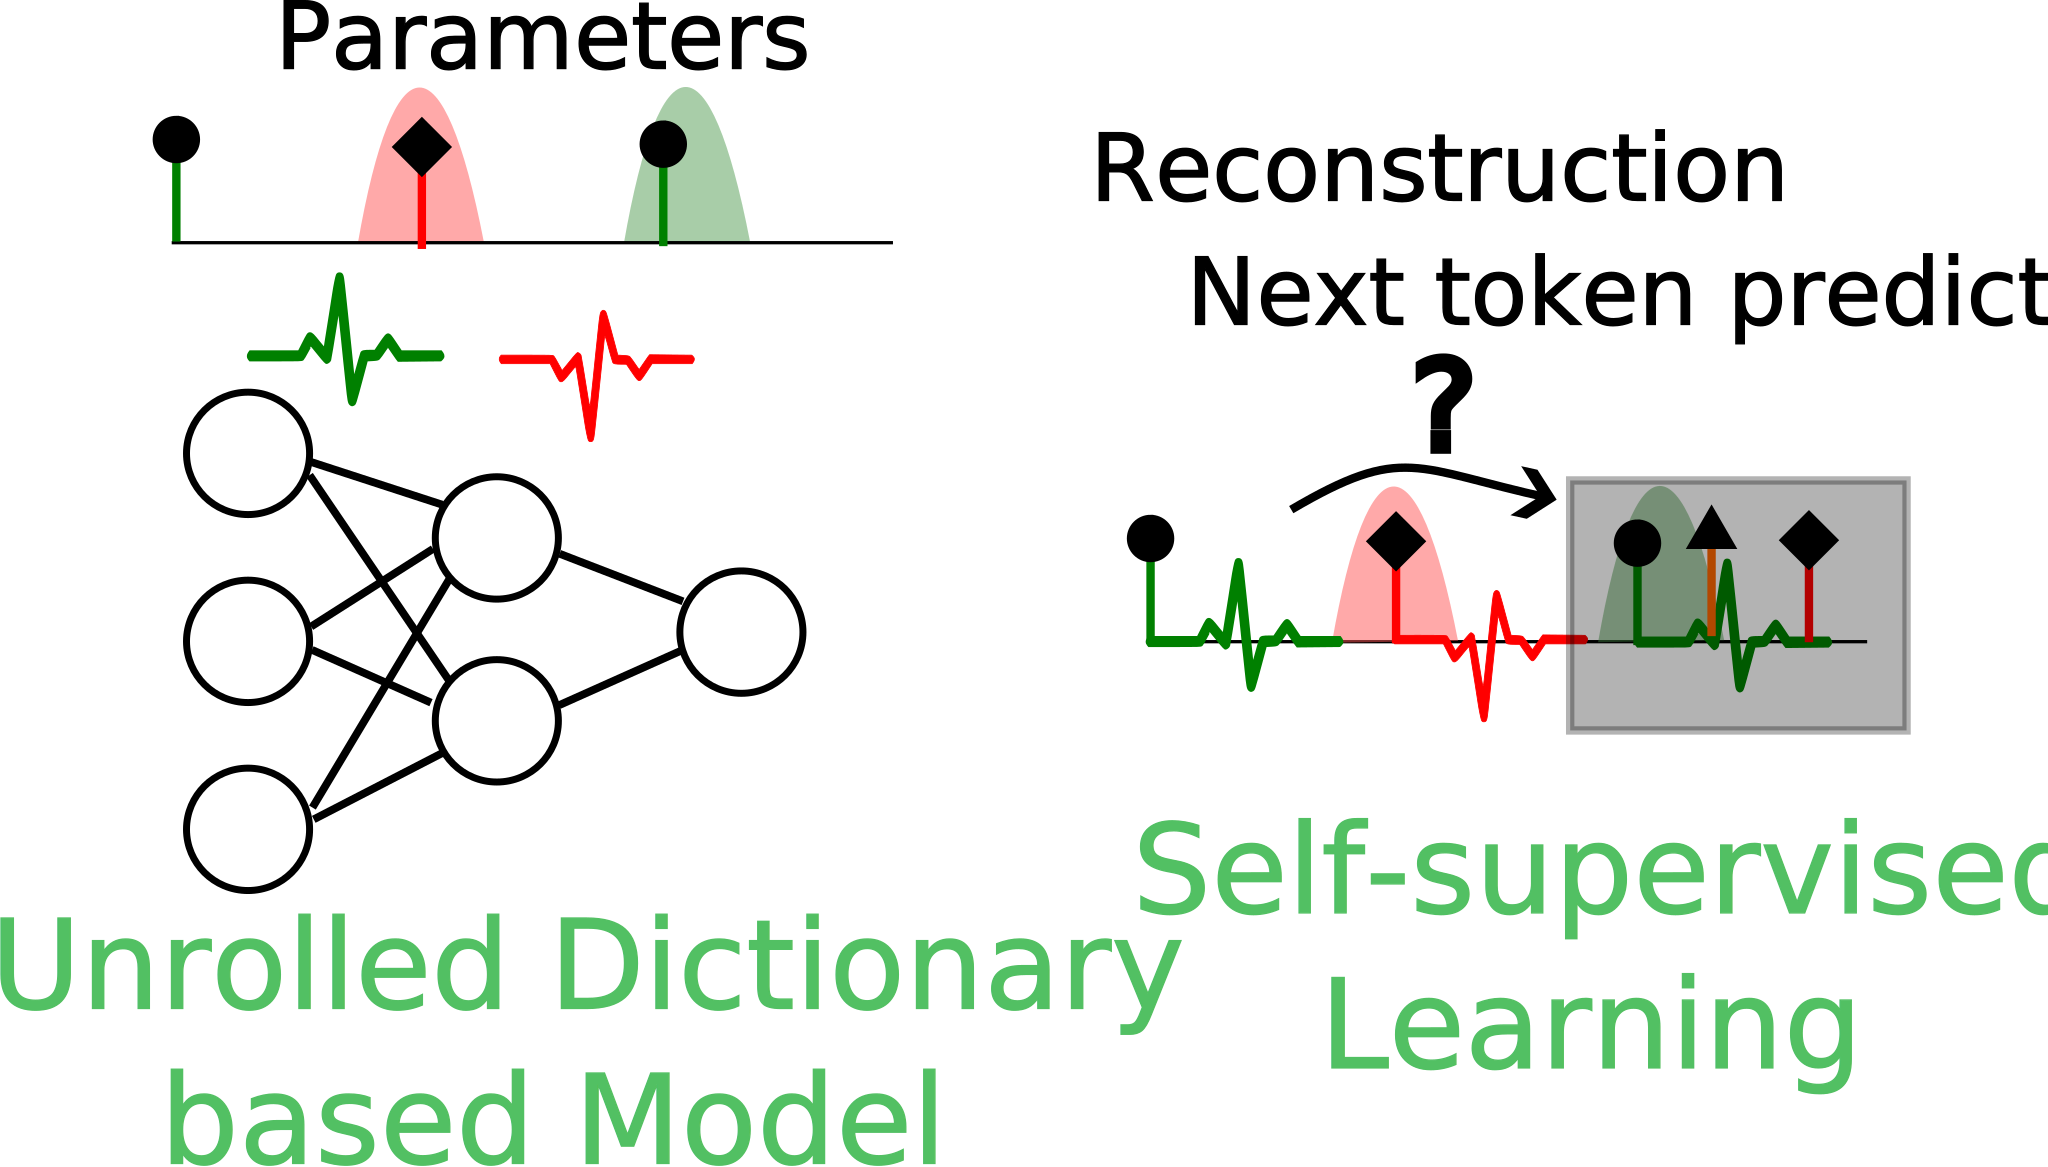
\includegraphics[width=.9\textwidth]{unrolled}};
        \end{tikzpicture}
        % \begin{itemize}
        %     \item Architecture based on parametric models unrolling,
        %     \item Fully differentiable.
        % \end{itemize}
    \end{columns}

    % \vskip2em
    % {\bf Expected Results:}\\[.5em]
    % \myitem{} Methods to build joint representations for signal and events.\hfill

    \vskip1em
    \definecolor{lightgreen}{RGB}{82,192,99}
    {\bf Preliminary Studies:} \fakecite{NeurIPS 2022; \textcolor{lightgreen}{ICLR 2022a}}
}

%------------------------------------------------------------------------------

\frame{
    \frametitle{WP3: Validating representations with practical tasks}

    \begin{block}{\bf Challenge 3}
        Can we develop methods based on event processing to impact GA?
    \end{block}

    \vskip1em
    % {\bf Expected Results:} Data processing for GA and Neurosciences.\\[1em]
    \begin{columns}[b]
        \column{.3\textwidth}
        \centering Detect adverse events in GA in real time.
        \vfill
        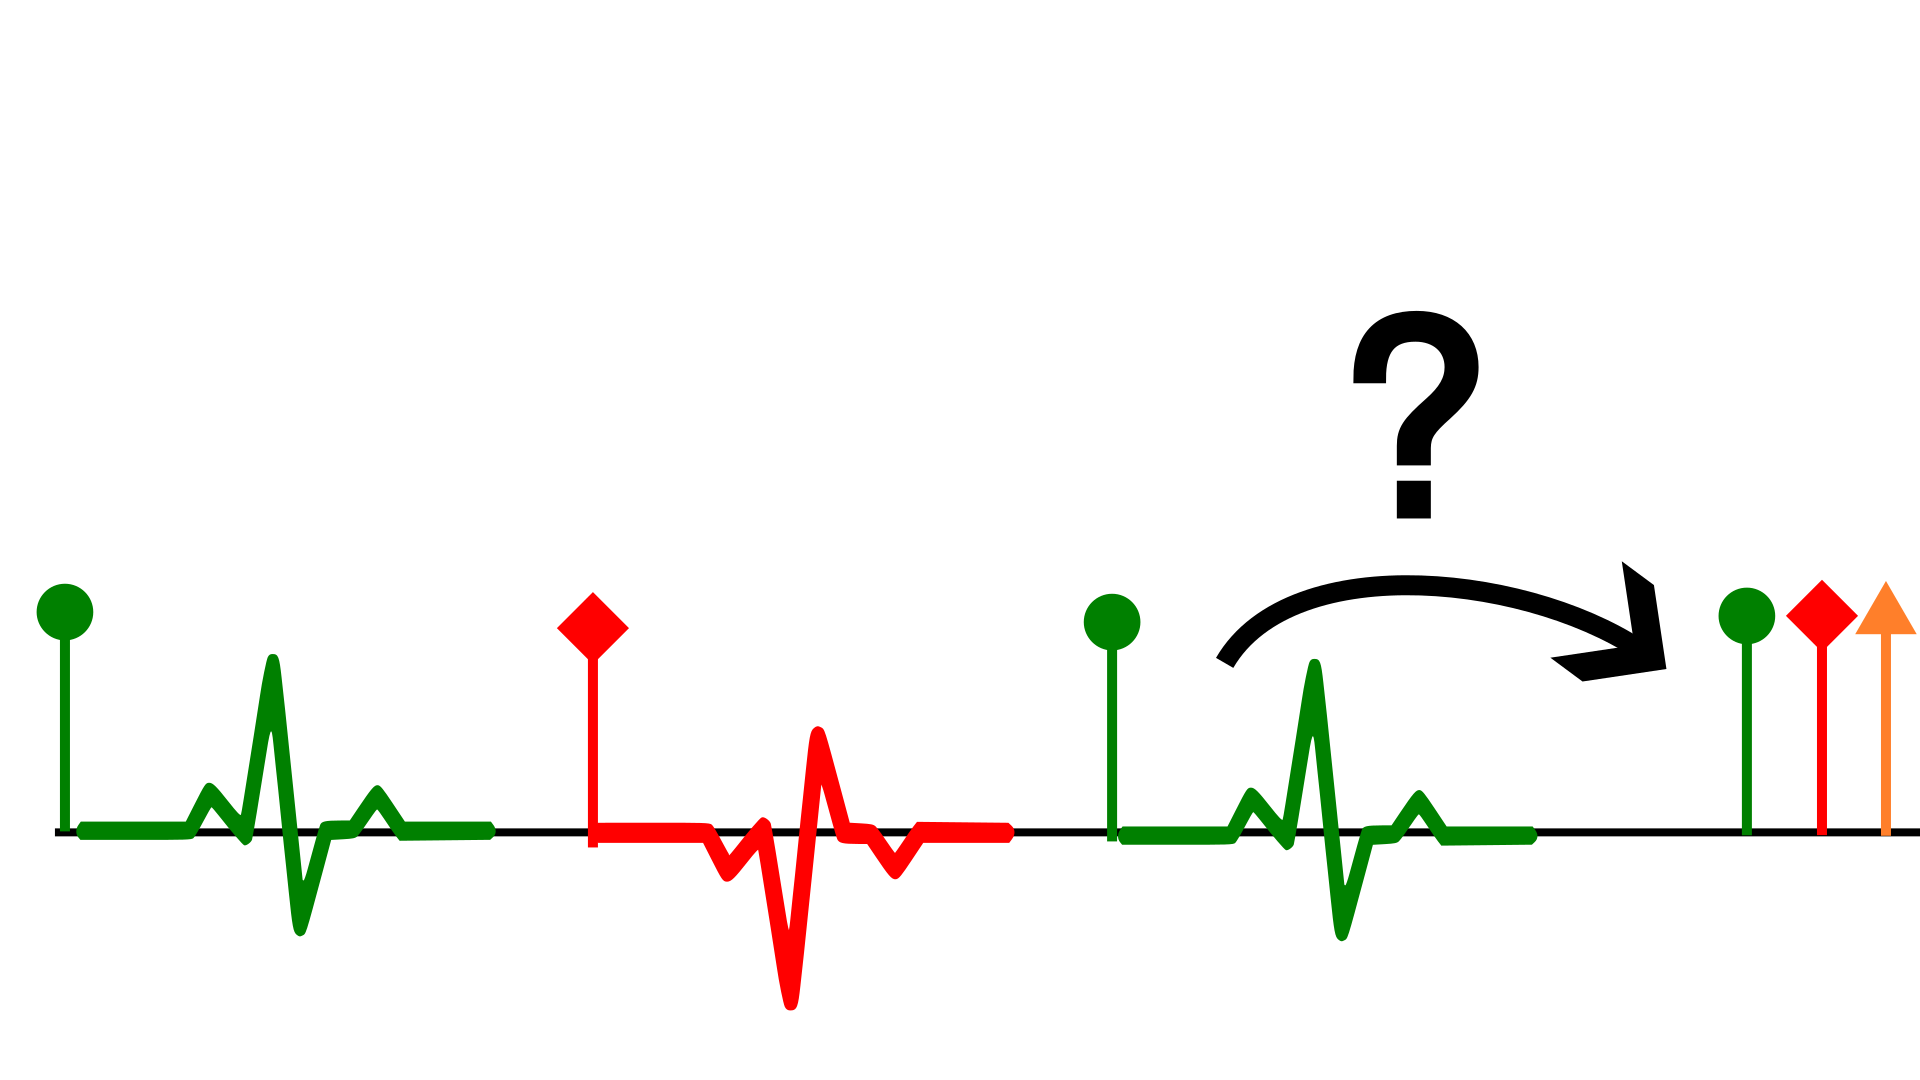
\includegraphics[width=\textwidth]{forecasting}
        \column{.3\textwidth}
        \centering Characterize abnormal records\vfill
        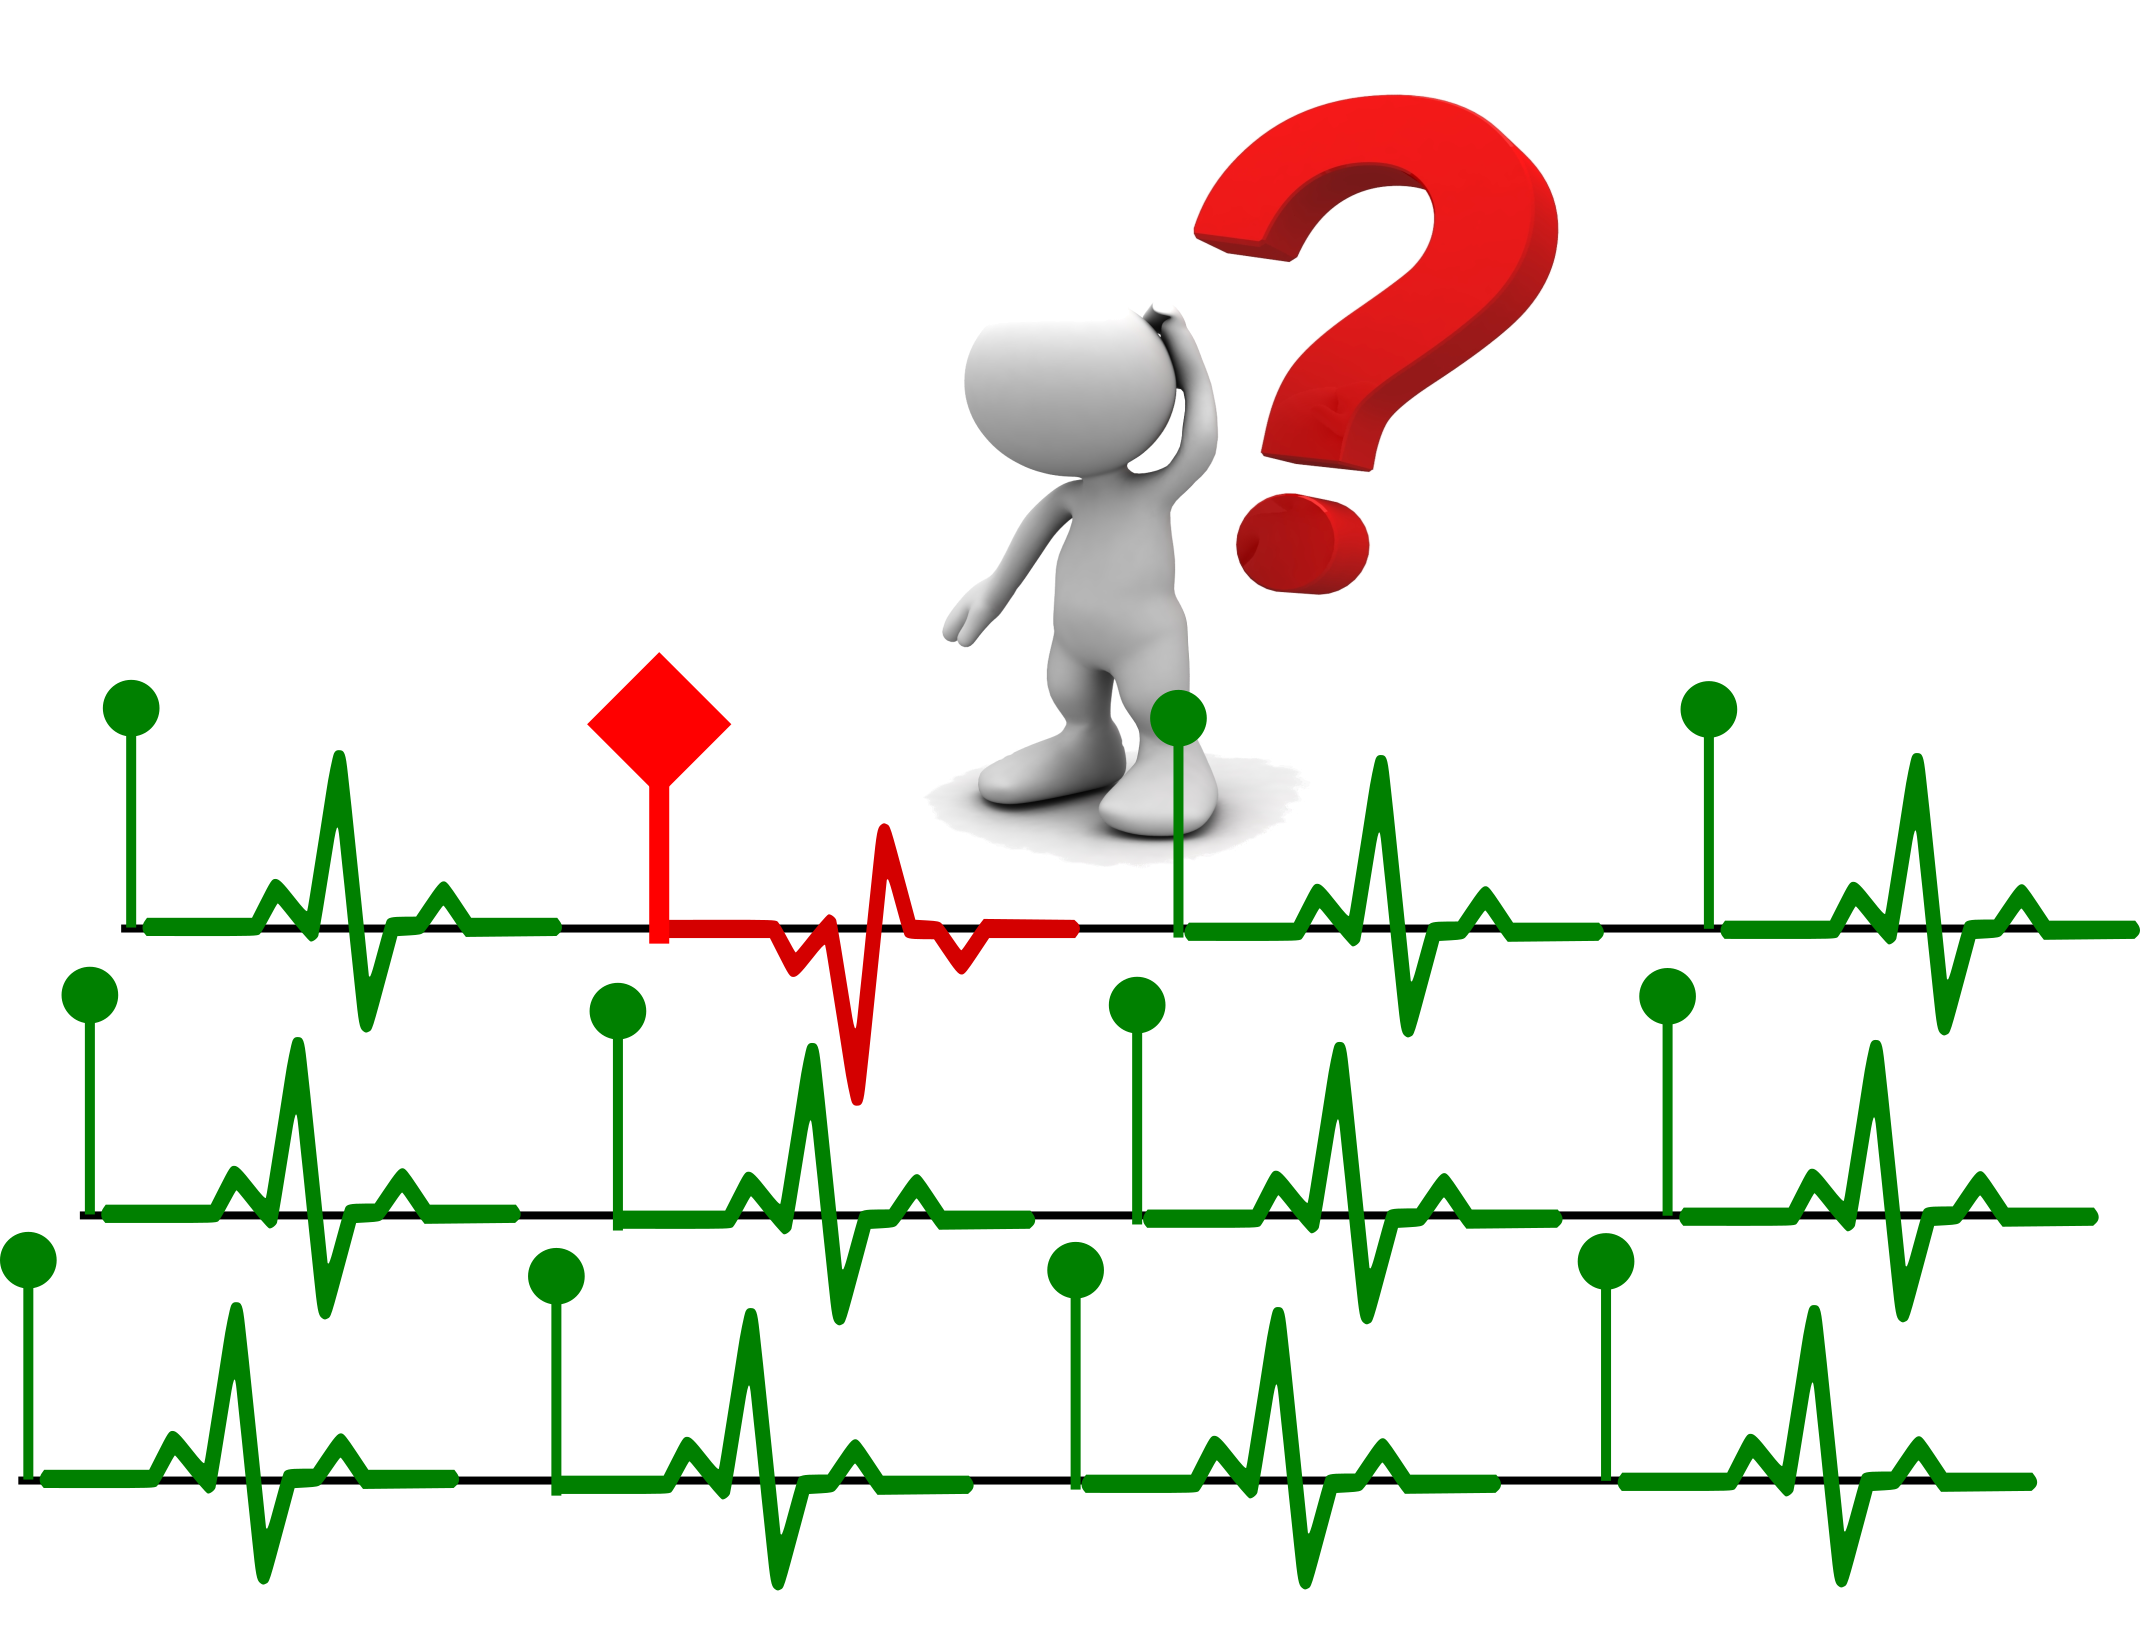
\includegraphics[width=1\textwidth]{anomaly_detection}
        \column{.3\textwidth}
        \centering Find causal relationship in Neuroscience.
        \vfill
        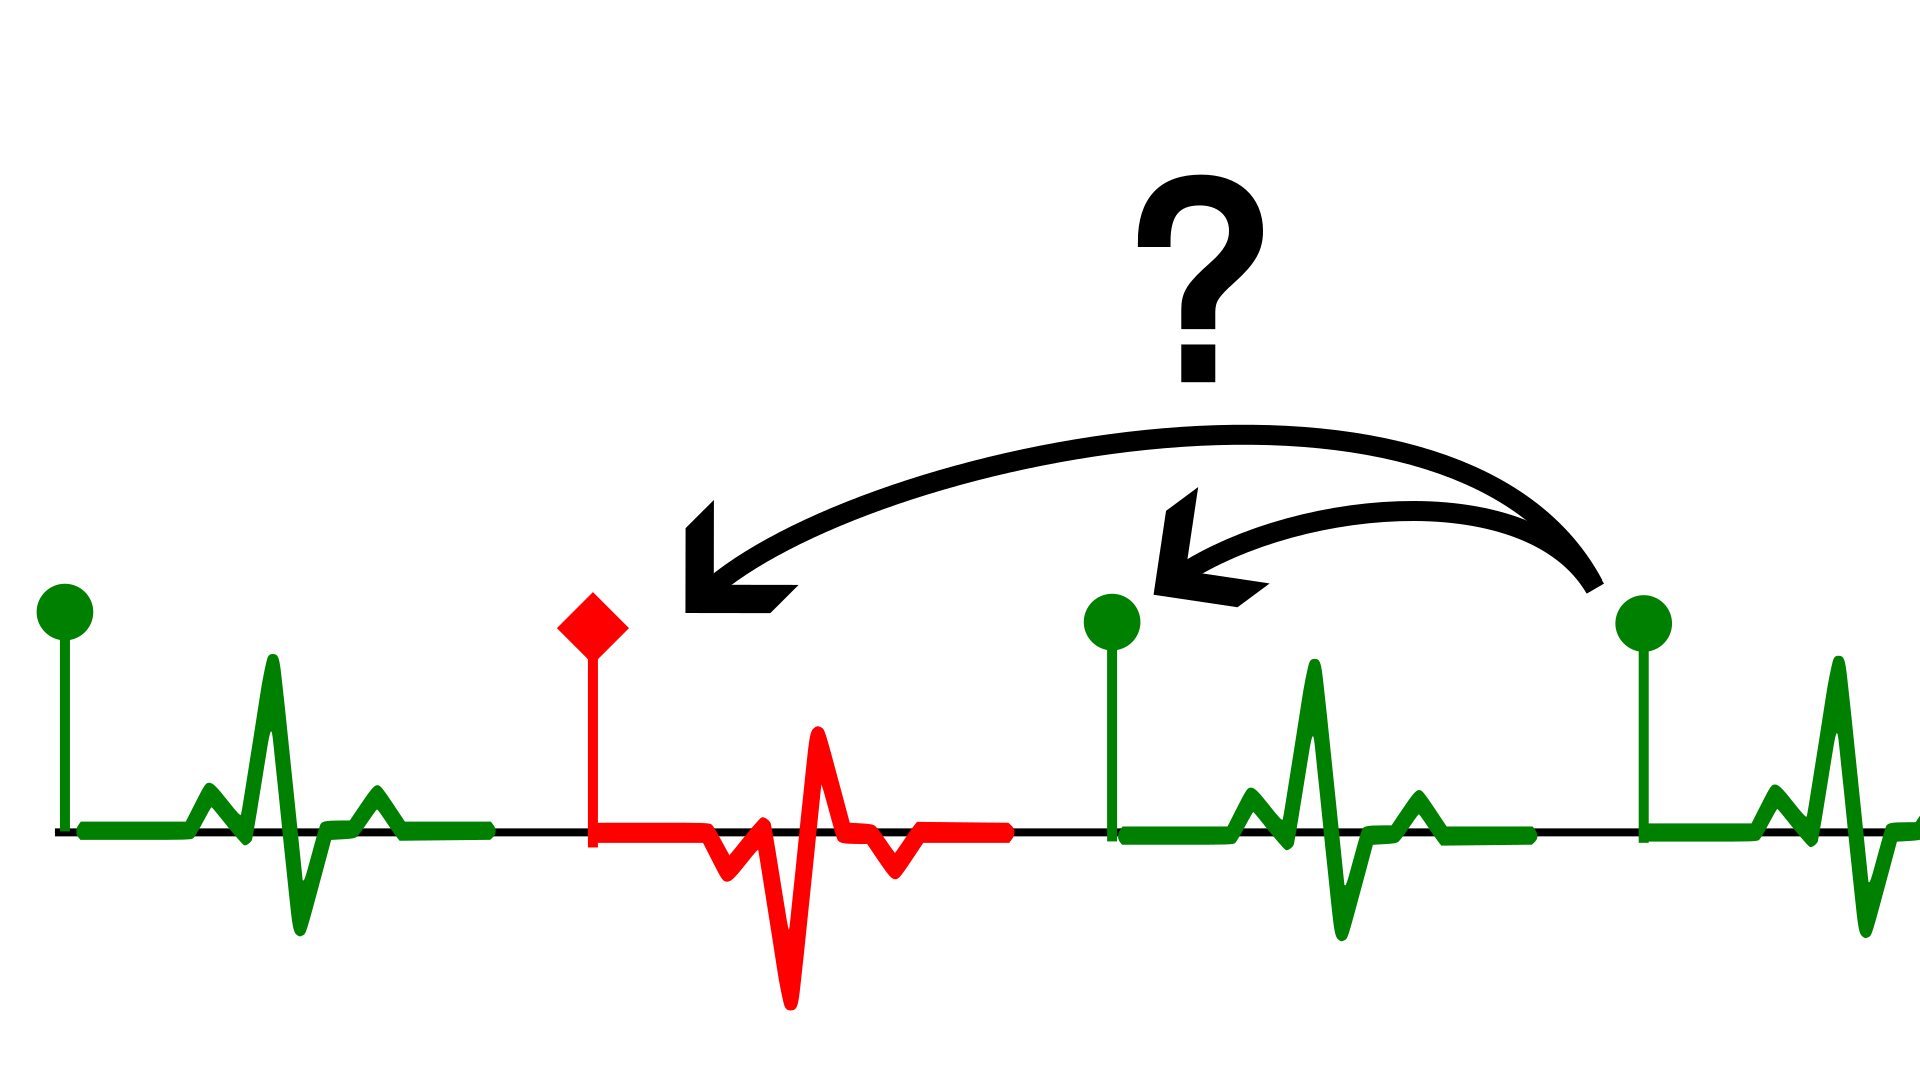
\includegraphics[width=\textwidth]{images/causality.png}
    \end{columns}
    % \vskip1em
    \begin{columns}[T]
        \techterm{Event Prediction}
        \techterm{Anomaly Detection}
        \techterm{Causality}
    \end{columns}

    \vskip1em
    {\bf Idea:} Leverage model likelihood and   differentiable architectures.

}

%------------------------------------------------------------------------------

% \frame{
%     \frametitle{WP4: Reproducible and Reusable Research}

%     \begin{block}{\bf Challenge 4}
%         Disseminate these techniques.
%     \end{block}

% }

%------------------------------------------------------------------------------

\frame[t]{
    \frametitle{EULPS: Event-based Unsupervised Learning for Physio. Data}

    % {\bf Carrier Path:}\\[.5em]
    % \highlightbox{\parbox{.9\textwidth}{
    %     \begin{tabular}{c p{2ex} l p{2ex} c}
    %         {\bf\color{black} 2014-2017}&&PhD && ENS Cachan\\
    %         {\bf\color{black} 2018-2019}&&Postdoc && Inria\\
    %         {\bf\color{black} 2019-Present}&&Research faculty&& Inria\\

    %     \end{tabular}

    % }}
    \highlight{
        \centering Goal: \normalfont\normalcolor
         Propose a new Signal Processing methodology based on Events.
    }

    % tikz figure with 3 circles linked with arrows going forward and backward and the the following text in each circle:
    % - Core ML
    %- Applications
    % - Software
    \setbeamercolor{dl}{fg=white,bg=darkred!50}
    \begin{tikzpicture}[overlay, remember picture]

        \node[anchor=south, yshift=4em, xshift=-1ex] at (current page.south) (cloud_soft) {
\includegraphics[width=15ex]{cloud}};
        \node[anchor=north, yshift=1.2em] at (cloud_soft) (Soft) {\parbox{.16\textwidth}{\centering Open\\ Source}};
        \node[anchor=south, yshift=2em] at (Soft.north) {\parbox{.15\textwidth}{\centering \bf \color{darkred} Thomas Moreau}};
        \node[anchor=south, xshift=-12ex, yshift=4em] at (Soft.north) (cloud_ML) {
\includegraphics[width=15ex]{cloud}};
        \node[anchor=north, yshift=.7em] at (cloud_ML) (ML) {Core ML\phantom{p}};
        \node[anchor=south, xshift=12ex, yshift=4em] at (Soft.north) (cloud_app) {
\includegraphics[width=15ex]{cloud}};
        \node[anchor=north, yshift=.3em] at (cloud_app) (App) {Impact};

        \draw[-latex] (cloud_app) to[bend right=5] node[above,rotate=60] {} (cloud_ML);
        \draw[-latex] (cloud_ML) to[bend right=5] node[above,rotate=60] {} (cloud_app);
        \draw[-latex] (cloud_app) to[bend right=5] node[above,rotate=60] {} (cloud_soft);
        \draw[-latex] (cloud_soft) to[bend right=5] node[above,rotate=60] {} (cloud_app);
        \draw[-latex] (cloud_soft) to[bend right=5] node[above,rotate=60] {} (cloud_ML);
        \draw[-latex] (cloud_ML) to[bend right=5] node[above,rotate=60] {} (cloud_soft);

        \node[anchor=east, xshift=-20ex, yshift=-8ex] at (cloud_soft.west) {\includegraphics[height=1.5em]{logo_python}};
        \node[anchor=east, xshift=-12ex, yshift=-8ex] at (cloud_soft.west) (sklearn){\includegraphics[height=1.5em]{logo_sklearn}};
        \node[anchor=south, xshift=-3ex, yshift=-1ex] at (sklearn.north) (contrib) {\footnotesize Contributor};
        \node[anchor=east, xshift=-1ex, yshift=0ex] at (cloud_soft.west) {\includegraphics[height=3em]{logo_joblib}};
        \node[anchor=east, xshift=-1ex, yshift=-7ex] at (cloud_soft.west) {\includegraphics[height=3em]{logo_loky}};
        \node[anchor=west, xshift=-1ex, yshift=1ex] at (cloud_soft.east) (benchopt) {\includegraphics[height=3em]{logo_benchopt}};
        \node[anchor=west, xshift=0ex, yshift=-6ex] at (cloud_soft.east) (alpha) {\includegraphics[height=3em]{brain_and_signals}};
        \node[anchor=north, yshift=1ex] at (alpha.south) {\footnotesize\texttt{{\color{orange}$\pmb\alpha$}csc}};


        \node[anchor=east, yshift=2em] at (cloud_ML.west) {
            \highlight{\parbox[c]{.18\textwidth}{
                2018-2023\\
                \normalfont\color{black} 17 papers in top ML conf.
            }}
        };

        % \node[anchor=south, xshift=-3ex, yshift=-1ex] at (cloud_app.north) {
        %     \includegraphics[height=2em]{logo_APHP}
        % };
        \node[anchor=south, yshift=0em, xshift=0ex] at (cloud_app.north) {
            \highlight{\parbox[c]{.25\textwidth}{
                GA Database\\
                \normalfont\color{black}
                46k records; 25Tb
            }}
        };
        \node[anchor=west, yshift=-.5em, xshift=-3ex] at (cloud_app.east) {
            \highlight{\parbox[c]{.22\textwidth}{
                Many Domains\\
                \normalfont \color{black}
                Neurosciences\\
                Exascale simu.\\
                Sensor networks
            }}
        };


        \node[anchor=south, yshift=.3em] at (contrib.north) {
            \highlight[col=dl, c=white]{\parbox{.17\textwidth}{
                \footnotesize \normalfont
                \centering {\bf Downloads:}\\
                26M/month
            }}
        };
        \node[anchor=west, xshift=-2ex, yshift=-2em] at (benchopt.east) {
            \highlight[col=dl, c=white]{\parbox{.15\textwidth}{
                \footnotesize \normalfont
                \centering{\bf Downloads:}\\
                1k/month
            }}
        };
        \node[anchor=north] at (cloud_soft.south) {
            
\includegraphics[height=1em]{github}~@tommoral
        };
    \end{tikzpicture}
}





\appendix

%------------------------------------------------------------------------------
\frame{
    \frametitle{References}

    \footnotesize
    \begin{itemize}\itemindent4em
        \item[\fakecite{ICLR2022}] Allain, C., Gramfort, A. \& {\bf Moreau, T.} \emph{DriPP: Driven Point Process to Model Stimuli Induced Patterns in M/EEF Signals.} in ICLR 2022.
        \item[\fakecite{ICLR2022a}] Malézieux, B., {\bf Moreau, T.} \& Kowalski, M. \emph{Understanding approximate and Unrolled Dictionary Learning for Pattern Recovery.} in ICLR 2022.
        \item[\fakecite{NeurIPS2022}] Dagréou, M., Ablin, P., Vaiter, S. \& {\bf Moreau, T.} \emph{A framework for bilevel optimization that enables stochastic and global variance reduction algorithms.} in NeurIPS 2022.
        \item[\fakecite{ICML2023}] Staerman, G., Allain, C., Gramfort, A. \& {\bf Moreau, T.} \emph{FaDIn: Fast Discretized Inference for Hawkes Processes with General Parametric Kernels.} in ICML 2023.
        \item[\fakecite{NImg 2023}] Power, L., Allain, C., {\bf Moreau, T.}, Gramfort, A. \& Bardouille, T. \emph{Using convolutional dictionary learning to detect task-related neuromagnetic transients and ageing trends in a large open-access dataset.} NeuroImage 2023.

    \end{itemize}
}


%------------------------------------------------------------------------------

\frame{
    \frametitle{EULPS}


    \begin{block}{\bf Goal}
        Model Physiological Signals as the distribution of its Events.
    \end{block}

    \vskip1em
    {\bf Road:} From Parametric to Deep Models.
    \vskip1em
    {\bf Impact:} Physiological \& Physical Signals Processing
    \vskip1em
    {\bf Applications:} General Anesthesia \& Neuroscience
    \vskip1em
    {\bf Team:}\\
    \myitem{} PI, 4 PhDs, 2 post doc, 1 engineer\\
    \myitem{} Local support: point process/bilevel optimization/anesthesia

}


% %------------------------------------------------------------------------------

% \frame{
%     \bibliography{library}
% }

\end{document}